% Options for packages loaded elsewhere
\PassOptionsToPackage{unicode}{hyperref}
\PassOptionsToPackage{hyphens}{url}
%
\documentclass[
]{article}
\usepackage{amsmath,amssymb}
\usepackage{iftex}
\ifPDFTeX
  \usepackage[T1]{fontenc}
  \usepackage[utf8]{inputenc}
  \usepackage{textcomp} % provide euro and other symbols
\else % if luatex or xetex
  \usepackage{unicode-math} % this also loads fontspec
  \defaultfontfeatures{Scale=MatchLowercase}
  \defaultfontfeatures[\rmfamily]{Ligatures=TeX,Scale=1}
\fi
\usepackage{lmodern}
\ifPDFTeX\else
  % xetex/luatex font selection
\fi
% Use upquote if available, for straight quotes in verbatim environments
\IfFileExists{upquote.sty}{\usepackage{upquote}}{}
\IfFileExists{microtype.sty}{% use microtype if available
  \usepackage[]{microtype}
  \UseMicrotypeSet[protrusion]{basicmath} % disable protrusion for tt fonts
}{}
\makeatletter
\@ifundefined{KOMAClassName}{% if non-KOMA class
  \IfFileExists{parskip.sty}{%
    \usepackage{parskip}
  }{% else
    \setlength{\parindent}{0pt}
    \setlength{\parskip}{6pt plus 2pt minus 1pt}}
}{% if KOMA class
  \KOMAoptions{parskip=half}}
\makeatother
\usepackage{xcolor}
\usepackage[margin=2.54cm]{geometry}
\usepackage{longtable,booktabs,array}
\usepackage{calc} % for calculating minipage widths
% Correct order of tables after \paragraph or \subparagraph
\usepackage{etoolbox}
\makeatletter
\patchcmd\longtable{\par}{\if@noskipsec\mbox{}\fi\par}{}{}
\makeatother
% Allow footnotes in longtable head/foot
\IfFileExists{footnotehyper.sty}{\usepackage{footnotehyper}}{\usepackage{footnote}}
\makesavenoteenv{longtable}
\usepackage{graphicx}
\makeatletter
\def\maxwidth{\ifdim\Gin@nat@width>\linewidth\linewidth\else\Gin@nat@width\fi}
\def\maxheight{\ifdim\Gin@nat@height>\textheight\textheight\else\Gin@nat@height\fi}
\makeatother
% Scale images if necessary, so that they will not overflow the page
% margins by default, and it is still possible to overwrite the defaults
% using explicit options in \includegraphics[width, height, ...]{}
\setkeys{Gin}{width=\maxwidth,height=\maxheight,keepaspectratio}
% Set default figure placement to htbp
\makeatletter
\def\fps@figure{htbp}
\makeatother
\setlength{\emergencystretch}{3em} % prevent overfull lines
\providecommand{\tightlist}{%
  \setlength{\itemsep}{0pt}\setlength{\parskip}{0pt}}
\setcounter{secnumdepth}{5}
\usepackage{booktabs}
\usepackage{longtable}
\usepackage{array}
\usepackage{multirow}
\usepackage{wrapfig}
\usepackage{float}
\usepackage{colortbl}
\usepackage{pdflscape}
\usepackage{tabu}
\usepackage{threeparttable}
\usepackage{threeparttablex}
\usepackage[normalem]{ulem}
\usepackage{makecell}
\usepackage{xcolor}
\ifLuaTeX
  \usepackage{selnolig}  % disable illegal ligatures
\fi
\usepackage{bookmark}
\IfFileExists{xurl.sty}{\usepackage{xurl}}{} % add URL line breaks if available
\urlstyle{same}
\hypersetup{
  pdftitle={ERCOT Load Forecasting},
  pdfauthor={Daniel Whitehead, Alex Lopez, Jessalyn Chuang},
  hidelinks,
  pdfcreator={LaTeX via pandoc}}

\title{\textbf{ERCOT Load Forecasting}}
\usepackage{etoolbox}
\makeatletter
\providecommand{\subtitle}[1]{% add subtitle to \maketitle
  \apptocmd{\@title}{\par {\large #1 \par}}{}{}
}
\makeatother
\subtitle{\url{https://github.com/alex-lopez70/ChuangWhiteheadLopez_ENV797_TSA_FinalProject/}}
\author{Daniel Whitehead, Alex Lopez, Jessalyn Chuang}
\date{}

\begin{document}
\maketitle

{
\setcounter{tocdepth}{3}
\tableofcontents
}
\listoffigures

\newpage

\section{Introduction and Motivation}\label{introduction-and-motivation}

Load growth used to be fairly stagnant and was managed by implementing
more efficiency measures (Walton, 2023). However, with innovation in
electrical technologies (EVs, heat pumps, etc.) and the introduction of
new load sources (crypto mining and data centers), electrical load has
skyrocketed in recent years. As a result, we need new and innovative
measures of responding to this load growth, such as demand response,
interconnection reform, among others. The ability to forecast load
growth is an interesting task, because there are both general trends
(growth in electric technologies, climate change, and increasing
electrification, among others) and seasonal trends (periodic variations
in energy demand and consumption) that impact load.

\section{Relevance and Objectives}\label{relevance-and-objectives}

In the US, ERCOT is a market witnessing tremendous load growth. In 2018,
summer peak load record was 69.5 GW, but in just 5 years, this record
was broken with a 16 GW increase, with the new record hitting 85.6 GW
(Wilson and Zimmerman, 2023). Moreover, ERCOT set a new winter demand
peak in February 2025 with load being above 80 GW for the first time,
similar figures usually seen in summer months, which highlights load
growth not being exclusive to the summer (Kleckner, 2025). A lot of this
can be attributed to crypto mining facilities, data centers, and
industrial electrification (Guo, 2025).

At the same time, ERCOT has had some really exciting developments, from
being the wholesale market with the greatest growth in solar PV and
battery storage, to having the fastest interconnection process out of
all the ISO/RTOs in the US, making ERCOT one of the most dynamic
electric wholesale markets in North America. These developments have all
helped ERCOT respond to load growth in the wake of extreme weather
events like Winter Storm Uri in 2021. In this context, being able to
better forecast load growth in ERCOT will help contribute to greater
innovation in policy and technology to support load growth while
continuing to reliably serve pre-existing load.

\section{Dataset Information}\label{dataset-information}

The ERCOT load dataset was collected from GridStatus.io, a website and
Python library that provides a uniform API for accessing electricity
supply, demand, and pricing data for the major ISOs in the United States
(\url{https://www.gridstatus.io/live}).

\subsection{Description}\label{description}

Using its ``Export Data'' tool, we queried hourly temperature and daily
load and fuel mix data for ERCOT from January 2017 to April 2025. Below
is a description of the data set retrieved:

\begin{table}[!h]
\centering\centering
\caption{\label{tab:unnamed-chunk-3}Data Set Description}
\centering
\begin{tabular}[t]{l|l|l|l}
\hline
 & Load & Temperature & Fuel Mix\\
\hline
\cellcolor{gray!10}{\textbf{Units}} & \cellcolor{gray!10}{MW} & \cellcolor{gray!10}{°F} & \cellcolor{gray!10}{MW}\\
\hline
\textbf{Frequency} & Daily & Hourly & Daily\\
\hline
\textbf{Subsets} &  & ERCOT Zone & Fuel (Coal and lignite, Hydro, Nuclear,
\cellcolor{gray!10}{                 Solar, Wind, Natural Gas)}\\
\hline
\end{tabular}
\end{table}

\newpage

\subsection{Data Wrangling}\label{data-wrangling}

The earliest available data for ERCOT fuel mix was from January 2017, so
we decided to retrieve load, temperature, and fuel mix data from January
2017 onwards. After importing each of these three data sets (daily
values except for temperature data) for the dates 1 January 2017 to 4
April 2025 and converting them to data frames, we created a new `Date'
column for each of the three date sets that converted the time given in
the `interval\_start\_local' to a YYYY-MM-DD format. Regarding the
temperature data, since it is hourly data divided by zone, we first
found the hourly average for each zone, then the daily average for each
zone, and finally we found the daily average using all the zones in
ERCOT by using rowMeans(), group\_by(), and summarise(). We split the
data into training and testing subsets: testing data encompasses the
last 365 days of data, while the rest was classified as the training
data.

Since we are working with higher frequency data with multiple
seasonalities, we are using the \texttt{msts} class from package
\texttt{forecast} to create time series objects for our daily data sets.
Unlike the ts() function, reserved for data exhibiting single
seasonality, the msts() function allows for non-integer frequency
specification. We therefore created eight time series objects, one for
load, one for temperature, and one for each of the fuels we are
analyzing, namely coal and lignite, hydro, nuclear, solar, wind, and
natural gas, with a `seasonal.period = c(7, 365.25)' for each. Below are
summaries of the data structures of each of the three wrangled data
frames (for load, temperature, and fuel mix) that were then used to
create time series objects by using msts():

\begin{longtable}[]{@{}lll@{}}
\caption{ERCOT Load Summary}\tabularnewline
\toprule\noalign{}
Variable & Description & Units \\
\midrule\noalign{}
\endfirsthead
\toprule\noalign{}
Variable & Description & Units \\
\midrule\noalign{}
\endhead
\bottomrule\noalign{}
\endlastfoot
interval\_start\_local & Start Time for the Day (Local) & Character \\
interval\_start\_utc & Start Time for the Day (UTC) & Character \\
interval\_end\_local & End Time for the Day (Local) & Character \\
interval\_end\_utc & End Time for the Day (UTC) & Character \\
load & Load (MW) & Numeric \\
Date & Date (YYYY-MM-DD) & Date \\
\end{longtable}

\begin{longtable}[]{@{}lll@{}}
\caption{ERCOT Daily Temperature Summary}\tabularnewline
\toprule\noalign{}
Variable & Description & Units \\
\midrule\noalign{}
\endfirsthead
\toprule\noalign{}
Variable & Description & Units \\
\midrule\noalign{}
\endhead
\bottomrule\noalign{}
\endlastfoot
Date & Date (YYYY-MM-DD) & Date \\
mean(Average) & Average Daily Temperature (°F) & Numeric \\
\end{longtable}

\begin{longtable}[]{@{}
  >{\raggedright\arraybackslash}p{(\columnwidth - 4\tabcolsep) * \real{0.3043}}
  >{\raggedright\arraybackslash}p{(\columnwidth - 4\tabcolsep) * \real{0.5507}}
  >{\raggedright\arraybackslash}p{(\columnwidth - 4\tabcolsep) * \real{0.1449}}@{}}
\caption{ERCOT Fuel Mix Summary}\tabularnewline
\toprule\noalign{}
\begin{minipage}[b]{\linewidth}\raggedright
Variable
\end{minipage} & \begin{minipage}[b]{\linewidth}\raggedright
Description
\end{minipage} & \begin{minipage}[b]{\linewidth}\raggedright
Units
\end{minipage} \\
\midrule\noalign{}
\endfirsthead
\toprule\noalign{}
\begin{minipage}[b]{\linewidth}\raggedright
Variable
\end{minipage} & \begin{minipage}[b]{\linewidth}\raggedright
Description
\end{minipage} & \begin{minipage}[b]{\linewidth}\raggedright
Units
\end{minipage} \\
\midrule\noalign{}
\endhead
\bottomrule\noalign{}
\endlastfoot
interval\_start\_local & Start Time for the Day (Local) & Character \\
interval\_start\_utc & Start Time for the Day (UTC) & Character \\
interval\_end\_local & End Time for the Day (Local) & Character \\
interval\_end\_utc & End Time for the Day (UTC) & Character \\
coal\_and\_lignite & Generation from Coal and Lignite (MW) & Numeric \\
hydro & Generation from Hydro (MW) & Numeric \\
nuclear & Generation from Nuclear (MW) & Numeric \\
solar & Generation from Solar (MW) & Numeric \\
wind & Generation from Wind (MW) & Numeric \\
natural\_gas & Generation from Natural Gas (MW) & Numeric \\
\end{longtable}

\section{Data Exploration}\label{data-exploration}

To better understand the dynamics of electricity consumption and
generation in the ERCOT region, we wanted to visualize our time series
data (using the autoplot() function). These visuals gave us insights
into long-term trends and seasonal patterns in ERCOT load, temperature,
and the evolving fuel mix. By looking at these trends, we could spot
times of high demand and see how temperature changes affect energy use.
We also noticed shifts in the fuel mix, showing how the region is moving
toward more sustainable energy sources.

\subsection{ERCOT Load}\label{ercot-load}

The ERCOT load has shown a steady increase from 2017 to 2025. This rise
reflects growing residential and industrial electricity consumption,
which could be attributed to population growth, economic development,
and infrastructure expansion across Texas. Seasonal fluctuations are
also apparent, with noticeable peaks during periods of extreme
temperatures, particularly in the summer and winter months.

\begin{figure}
\centering
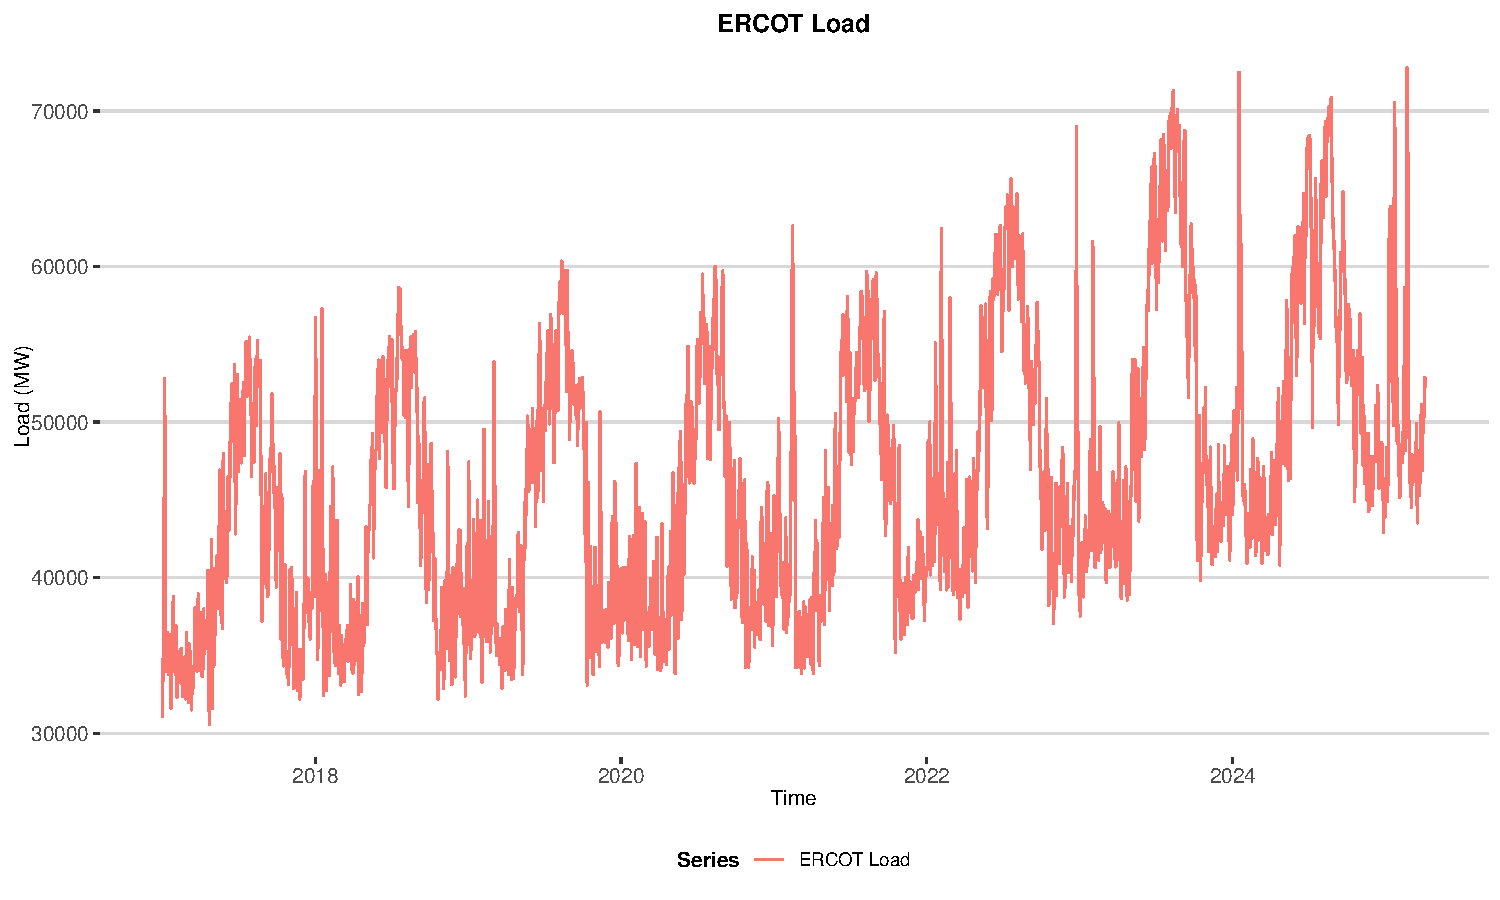
\includegraphics{FinalProject_Report_files/figure-latex/TS ERCOT Load Plot-1.pdf}
\caption{ERCOT Load from January 2017 to April 2025}
\end{figure}

The ACF of the ERCOT load series shows a slow decay, suggesting
non-stationarity and a strong trend over time. The irregular PACF, with
spikes at various lags, points to the seasonal components in the data,
and it gives some insight into how seasonality can be incroporated into
an auto-regressive model. The results of the ACF and PACF plots align
with our visualizations, which reveal a steady rise in load from 2017 to
2025 and clear seasonal peaks during periods of extreme temperatures.
These patterns show the impact of long-term growth and seasonal demand
shifts in Texas's electricity consumption.

\begin{figure}
\centering
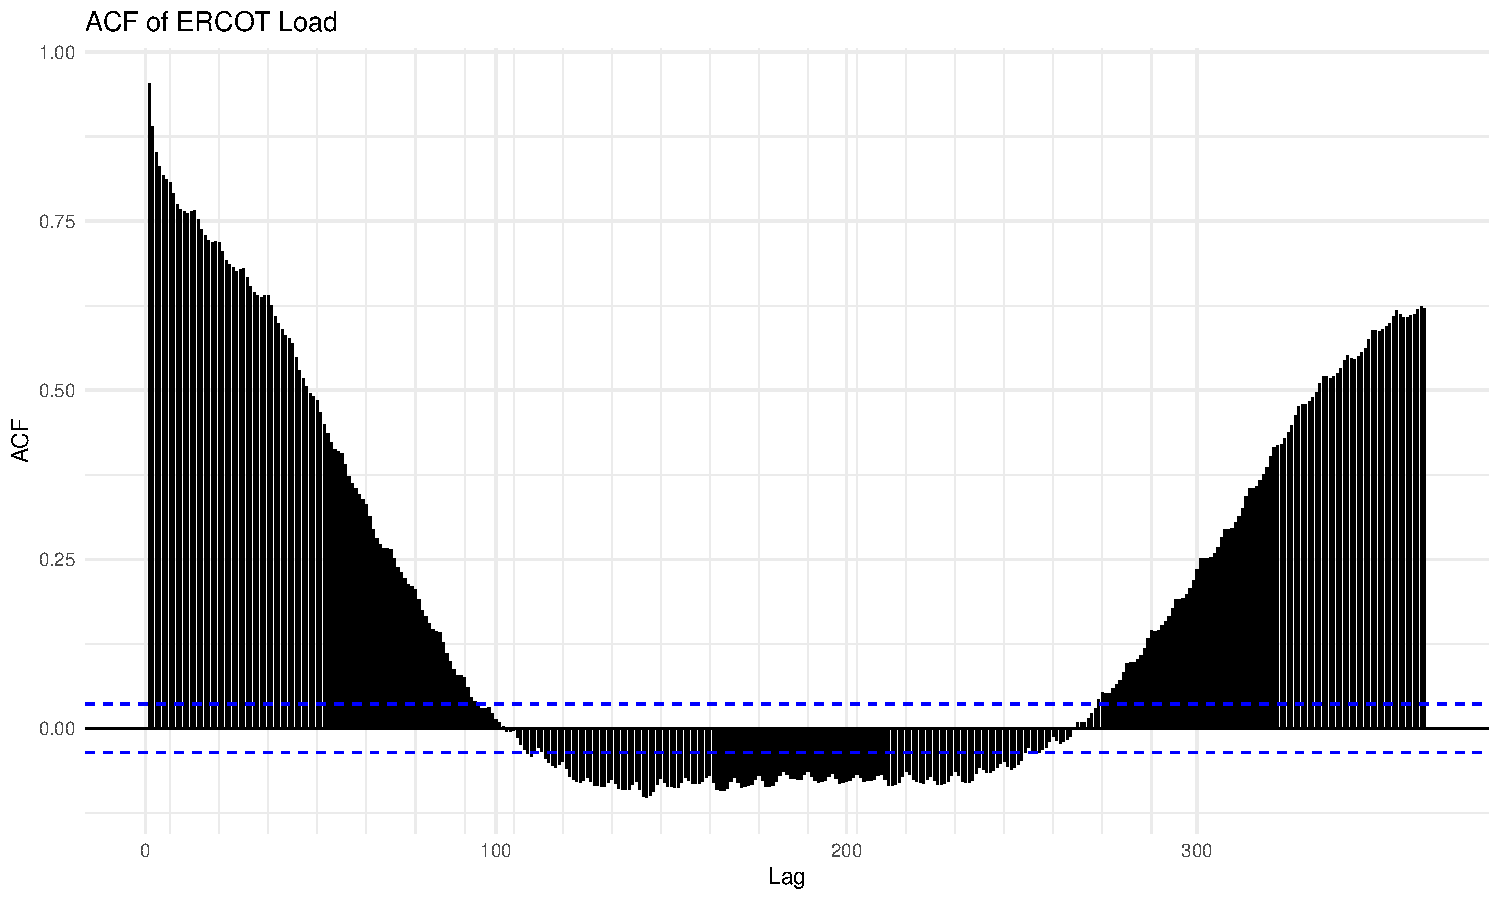
\includegraphics{FinalProject_Report_files/figure-latex/Load ACF-1.pdf}
\caption{ACF for Load}
\end{figure}

\begin{figure}
\centering
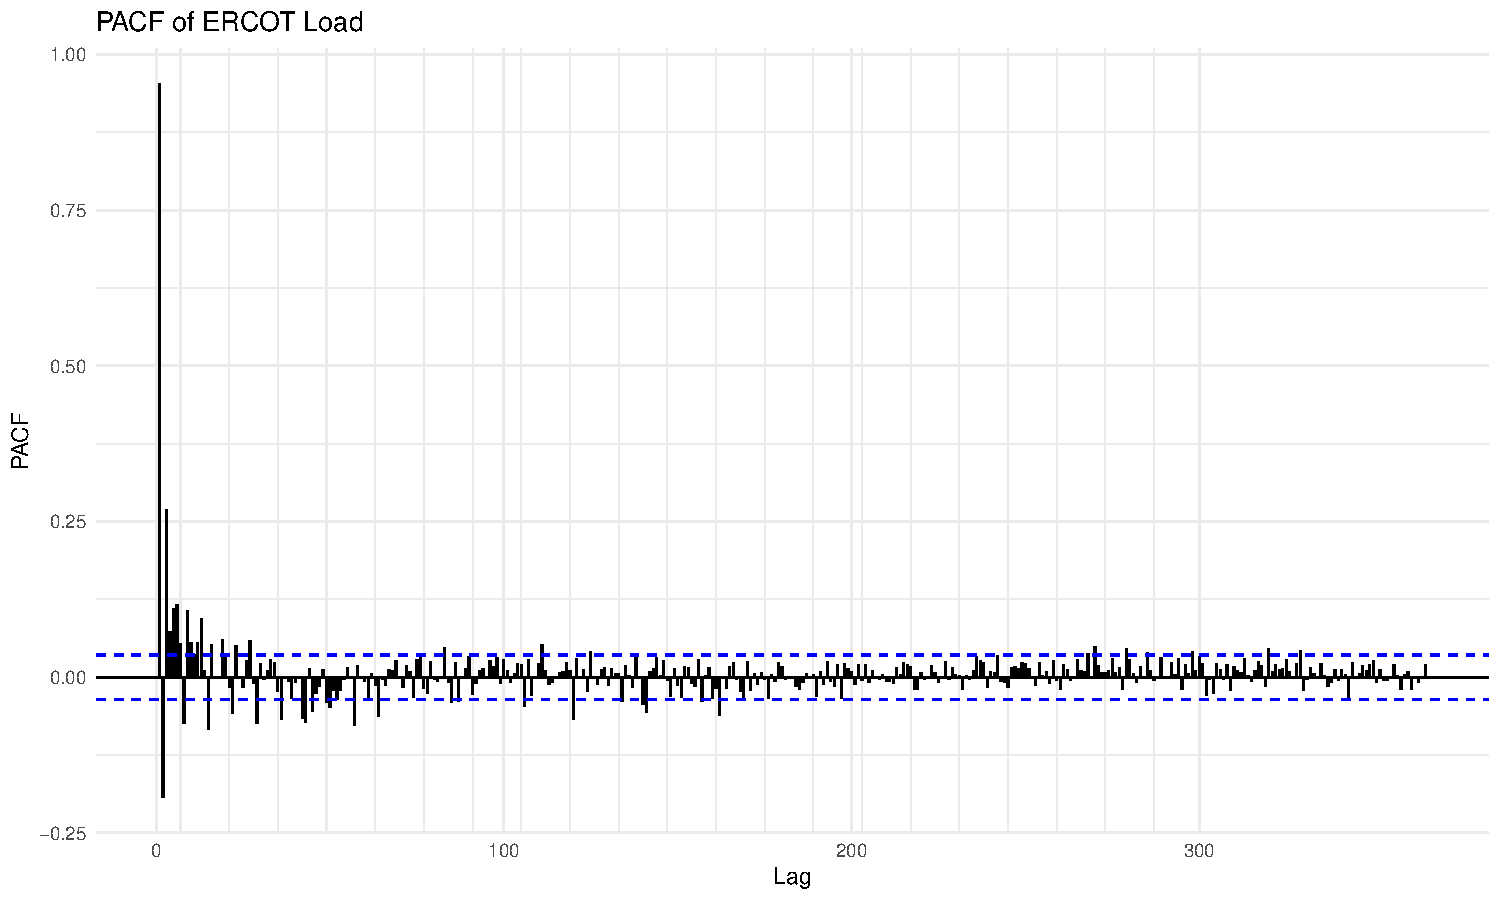
\includegraphics{FinalProject_Report_files/figure-latex/Load PACF-1.pdf}
\caption{PACF for Load}
\end{figure}

\newpage

\subsection{ERCOT Temperature}\label{ercot-temperature}

The temperature data was averaged daily for each zone and then combined
to get an overall ERCOT-wide daily average. This change helped us match
the temperature data with load and fuel mix data. As expected,
temperature patterns showed strong seasonality, with summer highs and
winter lows corresponding to fluctuations in load.

\begin{figure}
\centering
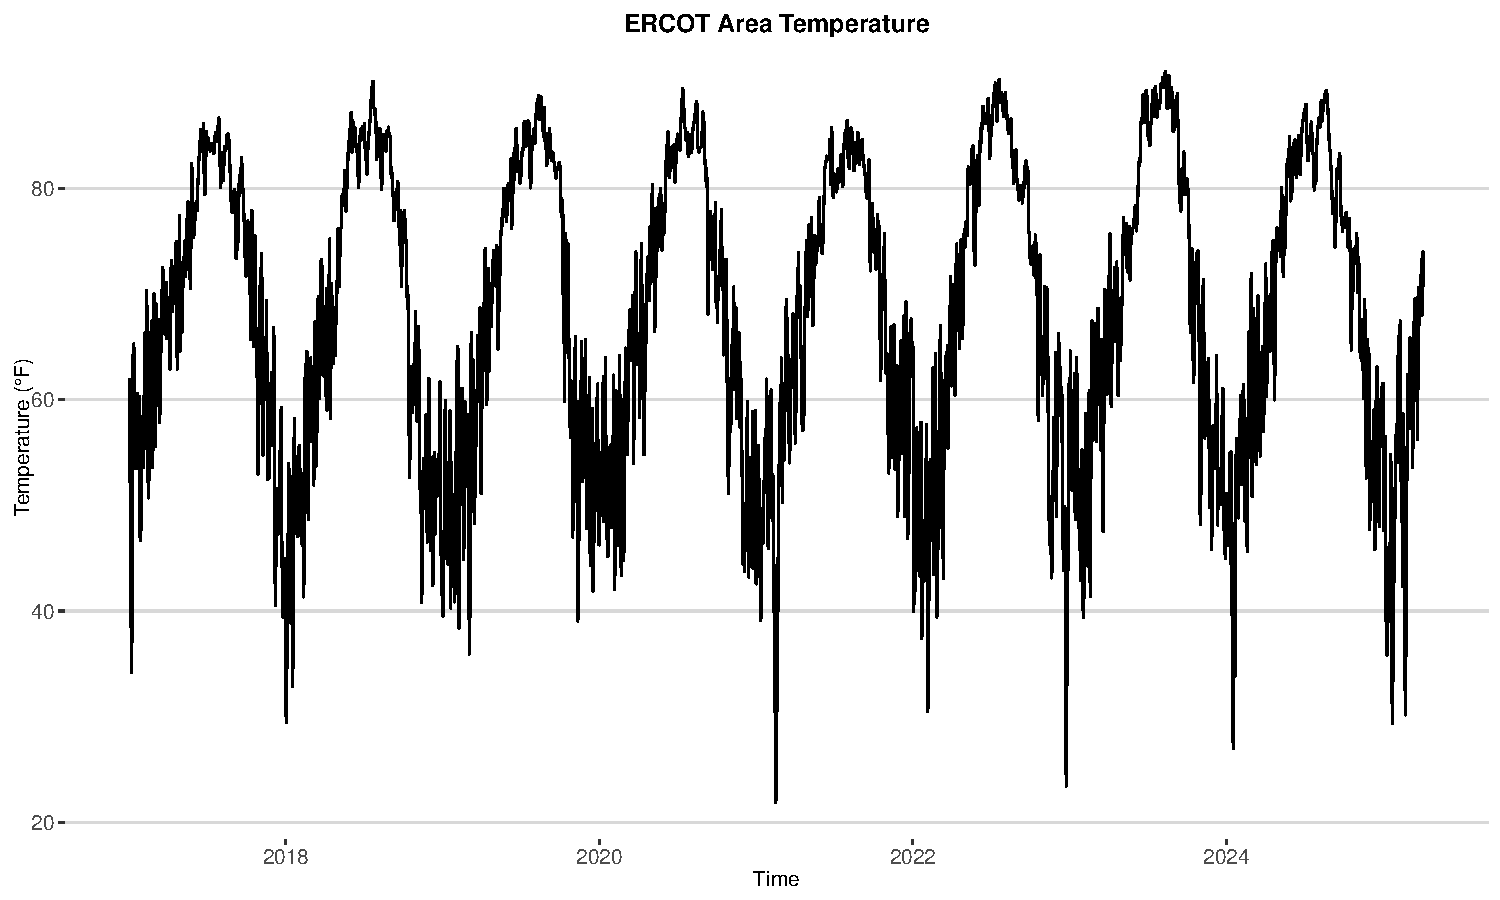
\includegraphics{FinalProject_Report_files/figure-latex/Temp TS-1.pdf}
\caption{ERCOT Temperature from January 2017 to April 2025}
\end{figure}

The ERCOT temperature series also exhibits a decaying ACF, indicating
non-stationarity and potential long-term trends in temperature over
time. The PACF of the temperature is similar to the PACF of the load,
with an initial short decay over the first 10 lags followed by scattered
significant spikes, suggesting both short-term autocorrelation and
possible seasonal components. These results seemed to match up with our
data for the ERCOT load, meaning it may have a significant role as an
exogenous variable in scenario generation.

\begin{figure}
\centering
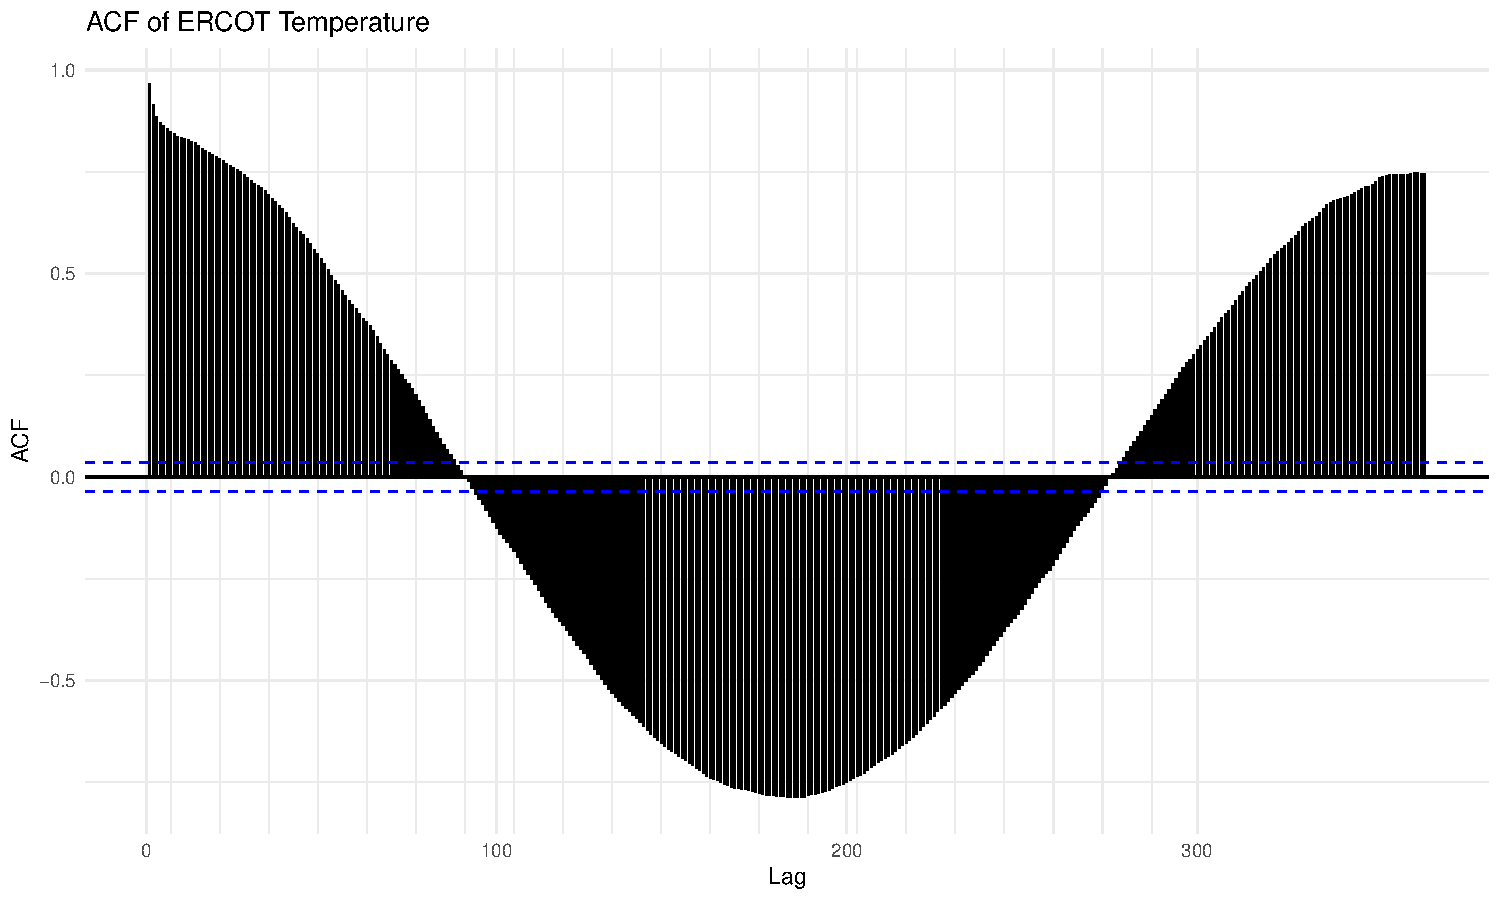
\includegraphics{FinalProject_Report_files/figure-latex/Temp ACF-1.pdf}
\caption{ACF for Temperature}
\end{figure}

\begin{figure}
\centering
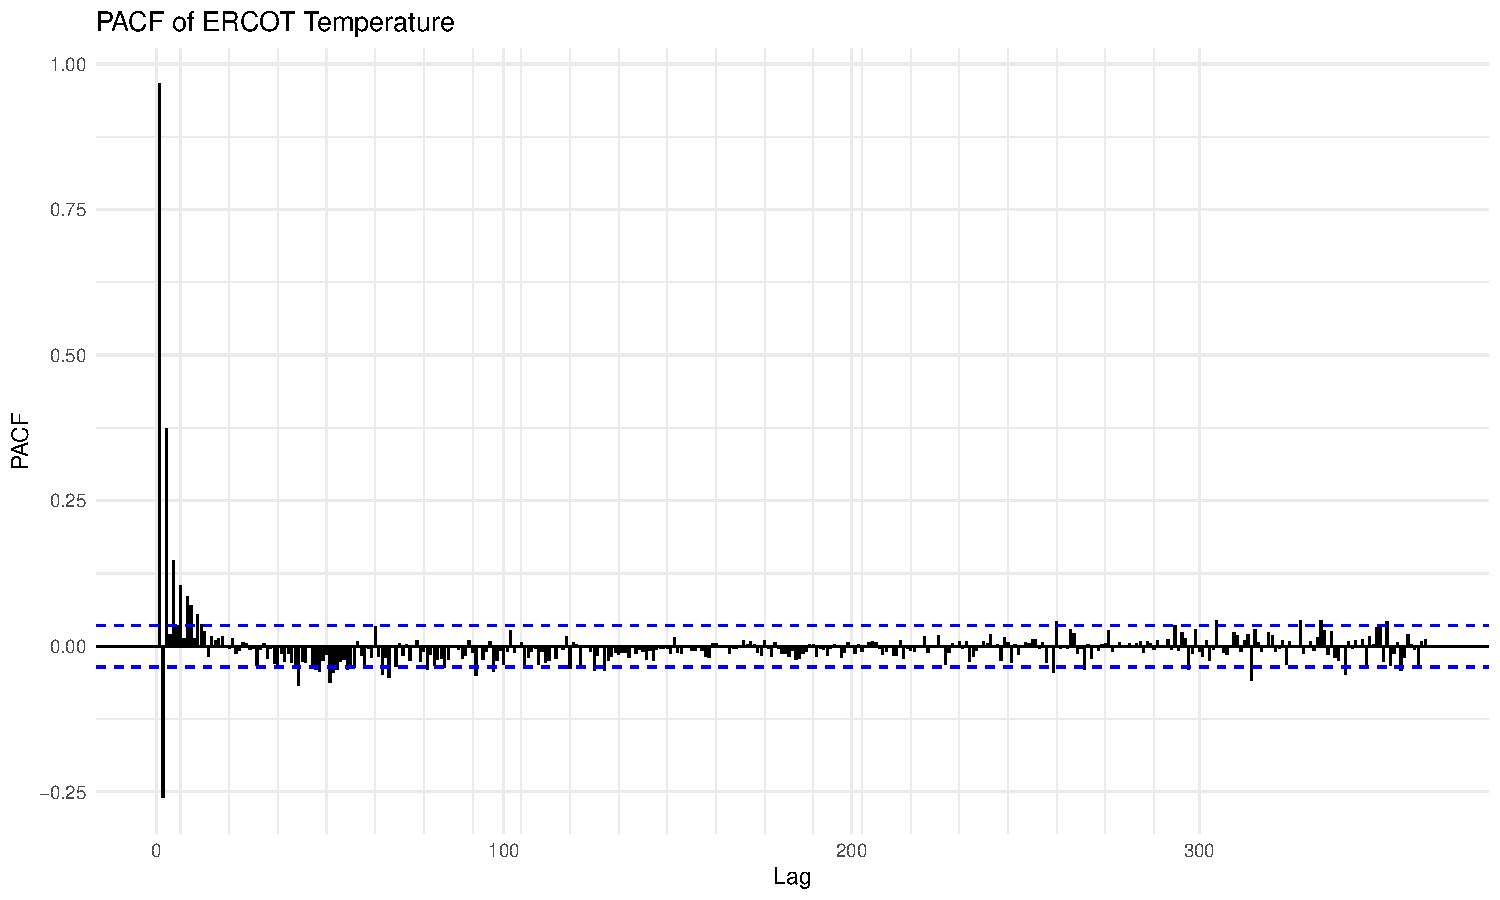
\includegraphics{FinalProject_Report_files/figure-latex/Temp PACF-1.pdf}
\caption{PACF for Temperature}
\end{figure}

\newpage

\subsection{ERCOT Fuel Mix}\label{ercot-fuel-mix}

ERCOT's fuel mix shows significant shifts over time. Natural gas seems
the most relevant and responsive energy source, as its load shape
closely mirrors the overall ERCOT demand curve. Coal and lignite usage
has declined steadily, and this aligns with national efforts to reduce
reliance on fossil fuels, as renewables such as wind and solar have
shown steady increase. ERCOT's nuclear generation and hydroelectric
power have both remained stable, though we should note that
hydroelectric has very minimal contribution to ERCOT's energy mix.

\begin{figure}
\centering
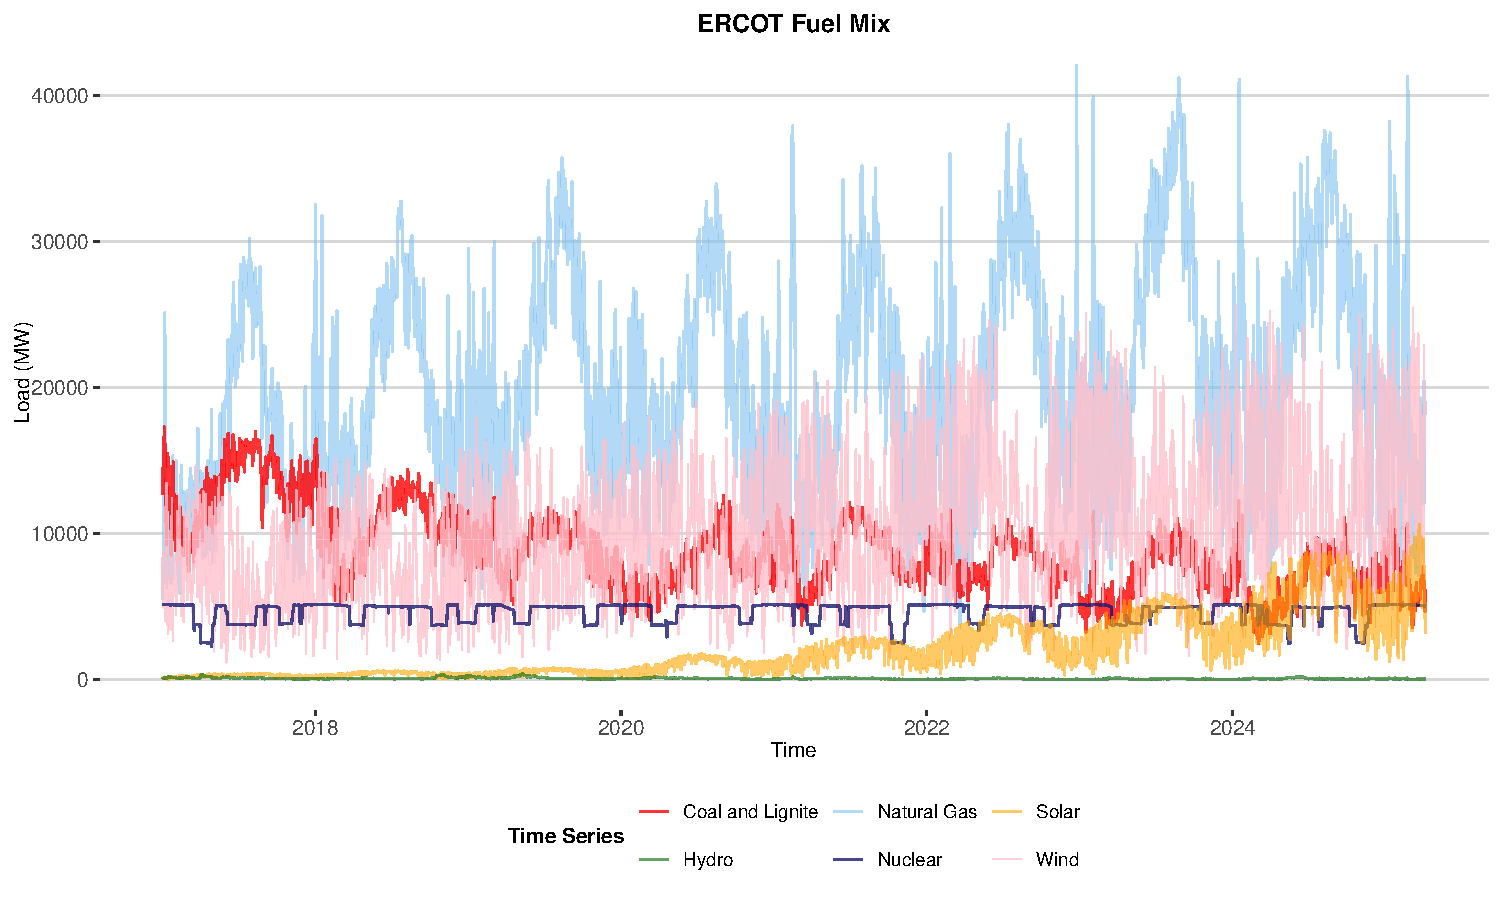
\includegraphics{FinalProject_Report_files/figure-latex/Plot TS Fuels-1.pdf}
\caption{ERCOT Fuel Mix from January 2017 to April 2025}
\end{figure}

Though all fuel mix ACFs and PACFs show non-stationary elements and
seasonal components, natural gas is the most applicable to display for
our ACF/PACF analysis, as the ACF and PACF of natural gas prices closely
resemble those of ERCOT load and temperature, showing a gradual decay in
the ACF and irregular spikes in the PACF. The shape of these plots
highlights the impact of natural gas in contributing to electricity
demand and makes it an important variable in scenario generation.

\begin{figure}
\centering
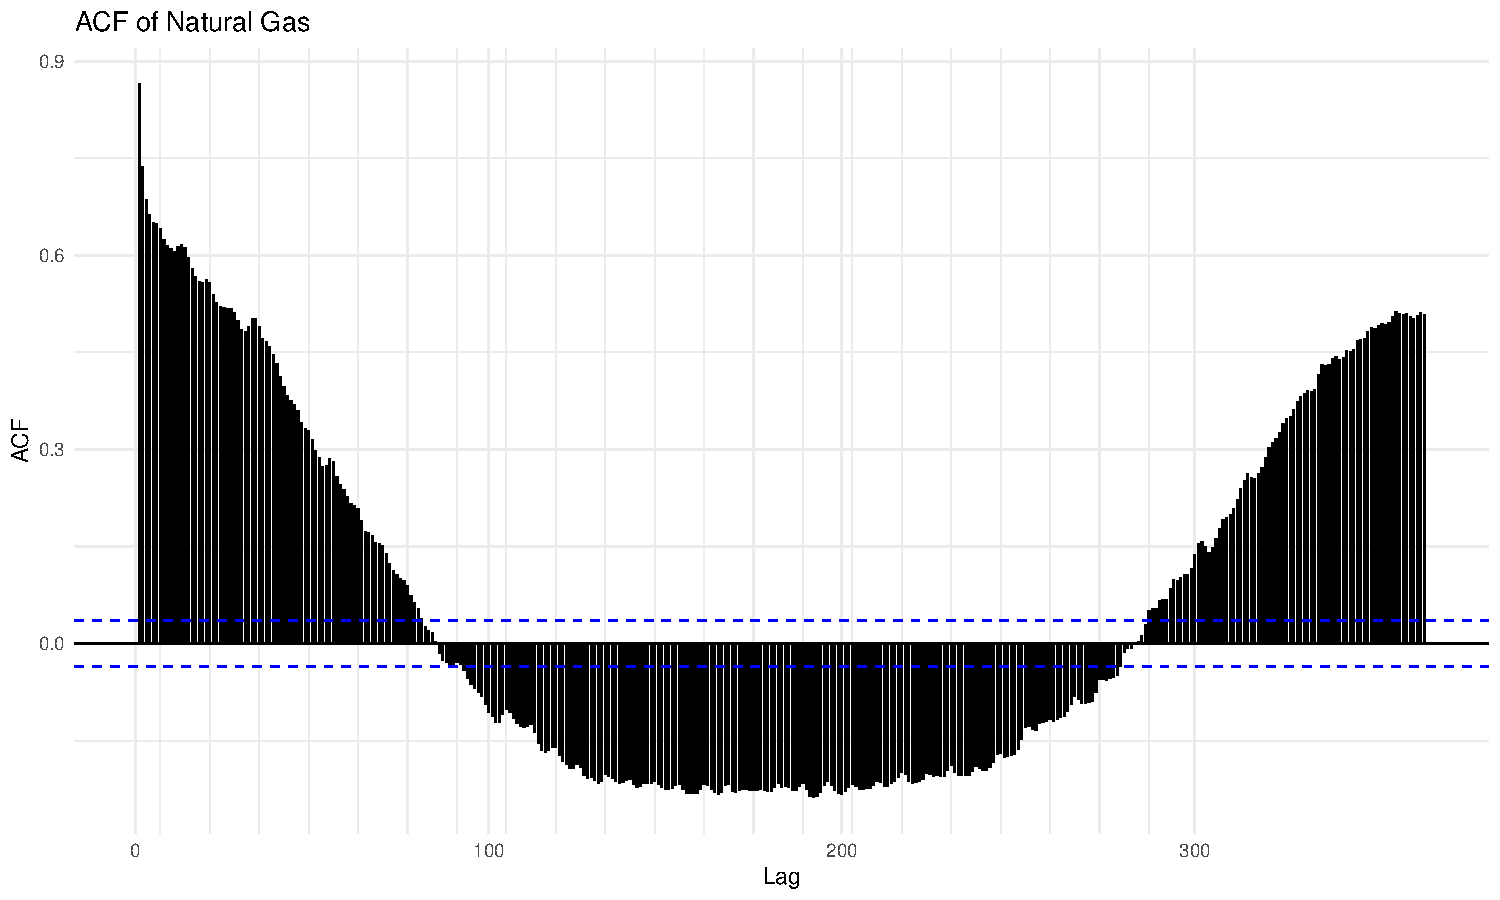
\includegraphics{FinalProject_Report_files/figure-latex/ACF for Natural Gas-1.pdf}
\caption{ACF for Natural Gas}
\end{figure}

\begin{figure}
\centering
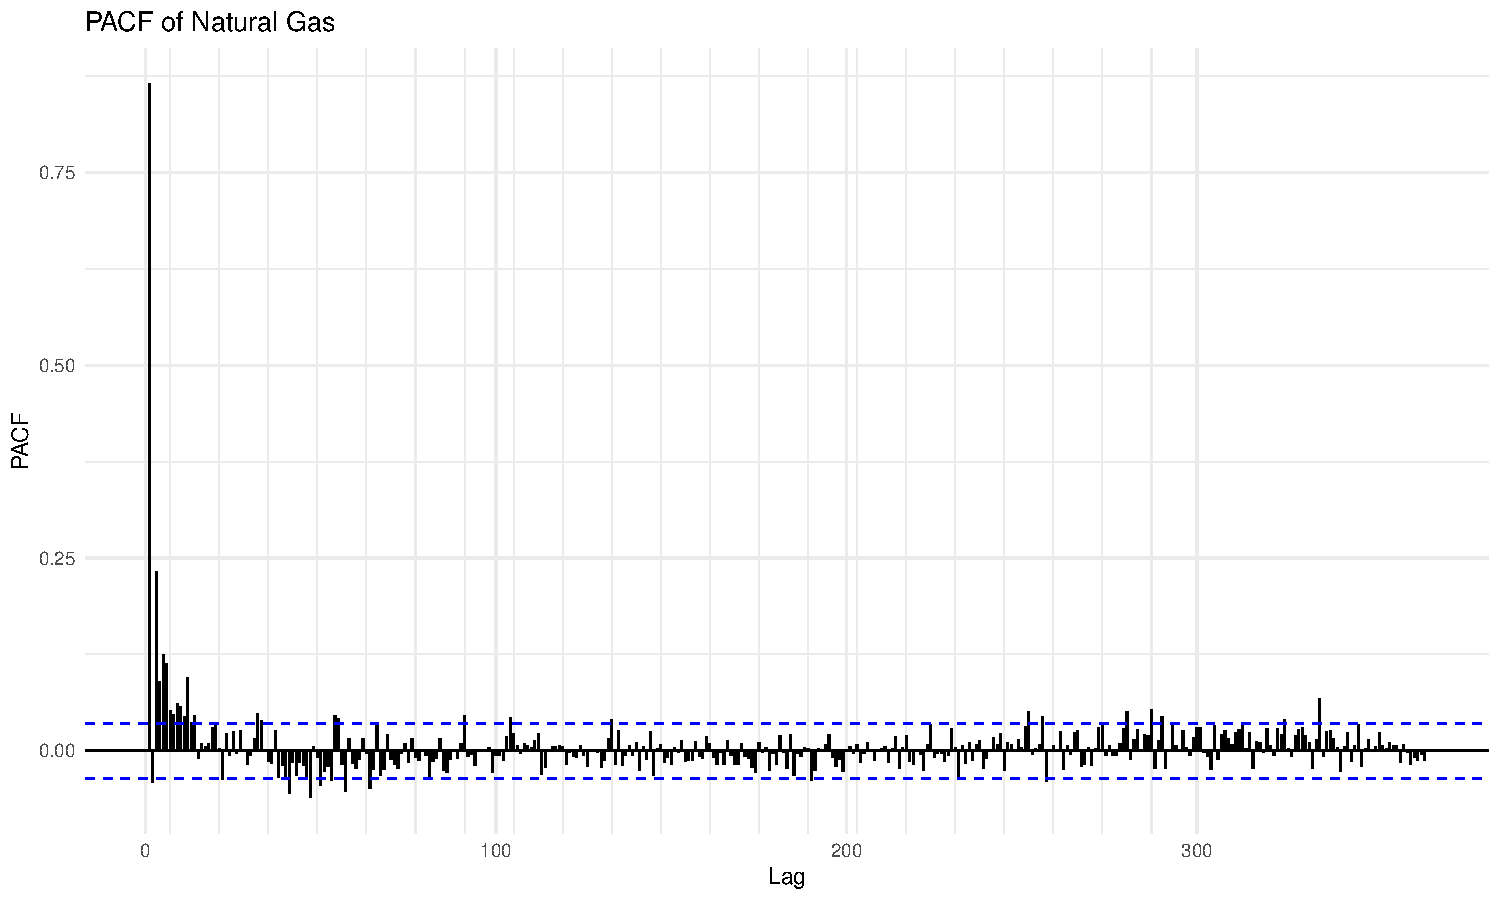
\includegraphics{FinalProject_Report_files/figure-latex/PACF for Natural Gas-1.pdf}
\caption{PACF for Natural Gas}
\end{figure}

\newpage

\section{Methodology and Models}\label{methodology-and-models}

Modeling ERCOT load is inherently complex due to the presence of
multiple seasonal patterns, non-linearities, and variability driven by
weather, human behavior, and market conditions. To capture these
dynamics, we used a varity of time series models, each offering unique
strengths.

\subsection{Models with Daily Data}\label{models-with-daily-data}

\subsubsection{STL + ETS}\label{stl-ets}

STL + ETS combines two powerful methods: Seasonal and Trend
decomposition using Loess (STL) and Exponential Smoothing (ETS). STL
decomposes the time series into its seasonal, trend, and remainder
components by using local smoothing techniques. Then, ETS applies
exponential smoothing to each of the seasonal, trend, and remainder
components to produce forecasts. This hybrid approach is particularly
effective for modeling complex and potentially evolving seasonal
patterns and trends in load data, as it allows the model to adapt to
changing dynamics over time. By separately forecasting each component,
it ensures better accuracy in the final forecast, especially when the
data exhibits smooth, but also varying, seasonality or trends.

\begin{figure}
\centering
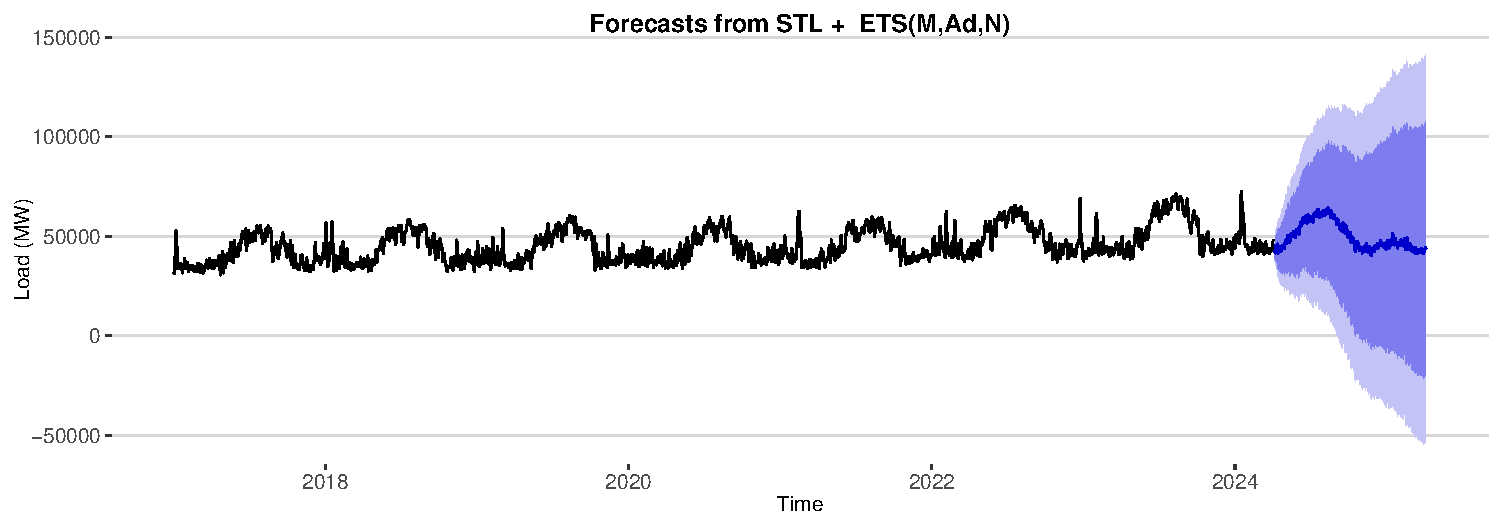
\includegraphics{FinalProject_Report_files/figure-latex/unnamed-chunk-4-1.pdf}
\caption{Forecasting Results from STL + ETS}
\end{figure}

\begin{figure}
\centering
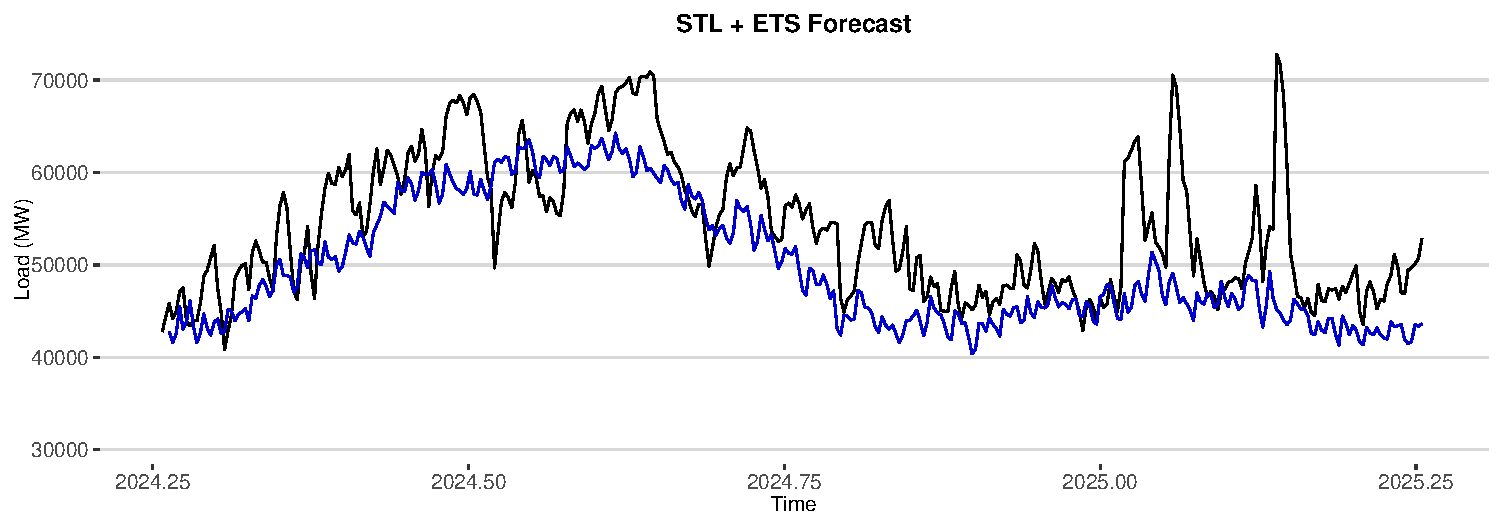
\includegraphics{FinalProject_Report_files/figure-latex/unnamed-chunk-5-1.pdf}
\caption{Observed Data and Forecasting Results from STL + ETS}
\end{figure}

\newpage

\subsubsection{TBATS}\label{tbats}

TBATS (Trigonometric Seasonalities, Box-Cox Transformation, ARMA Errors,
Trend, and Seasonal Components) is well-suited for modeling ERCOT load
due to its ability to capture multiple and non-integer seasonalities,
such as daily and weekly cycles, as well as complex seasonal
interactions. The model's flexibility in handling complex patterns and
its scalability for longer-term forecasts make it a valuable method for
accurate long-term load forecasting in dynamic systems like ERCOT.

\begin{figure}
\centering
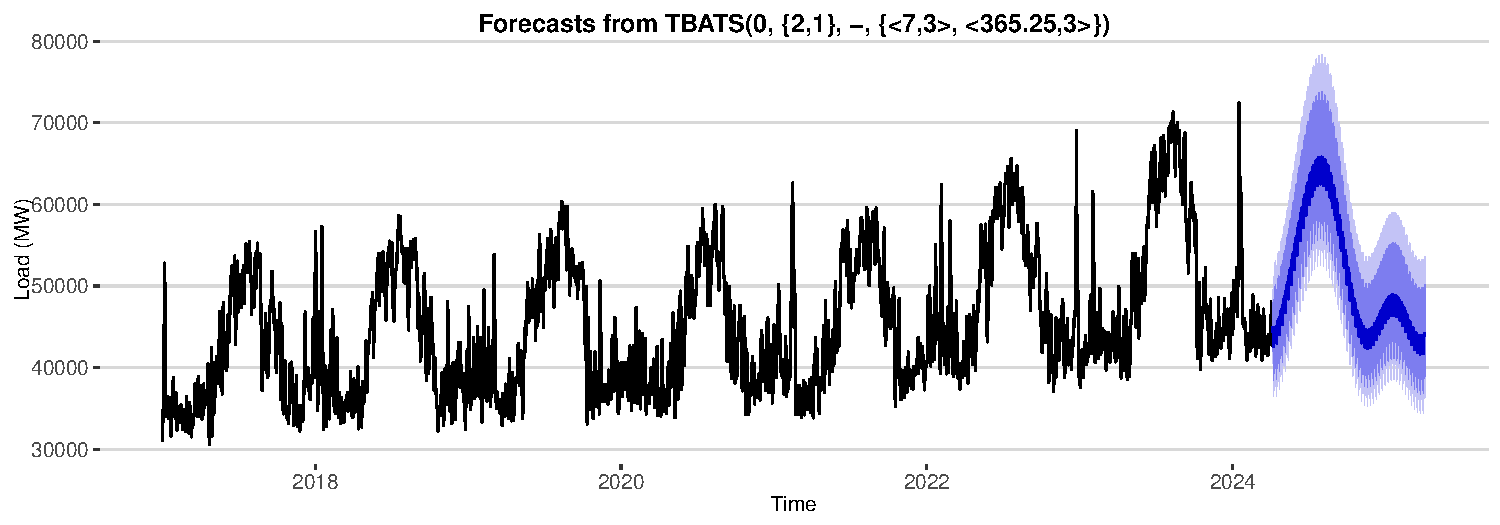
\includegraphics{FinalProject_Report_files/figure-latex/unnamed-chunk-6-1.pdf}
\caption{Forecasting Results from TBATS}
\end{figure}

\begin{figure}
\centering
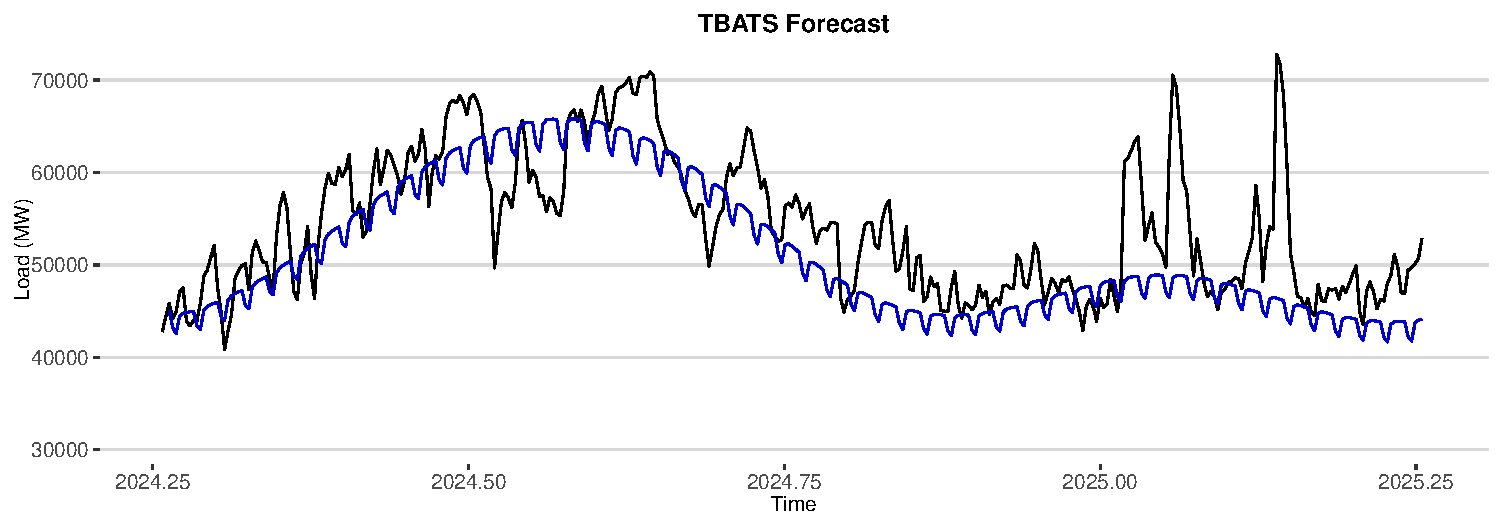
\includegraphics{FinalProject_Report_files/figure-latex/unnamed-chunk-7-1.pdf}
\caption{Observed Data and Forecasting Results from TBATS}
\end{figure}

\newpage

\subsubsection{ARIMA + Fourier Terms}\label{arima-fourier-terms}

This method integrates traditional autoregressive modeling with Fourier
terms as exogenous regressors, effectively capturing recurring seasonal
patterns like daily temperature-related demand fluctuations. This
approach enhances ARIMA's forecasting performance for load data by
explicitly modeling periodicities without the need for differencing
seasonal components.

Since the ARIMA + Fourier terms model is a good option for modeling
multiple seasonalities, we ran a few models with a variety of K
parameters. K is a vector of integers specifying the number of sine and
cosine terms for each of the seasonal periods. For our four ARIMA +
Fourier models, we used the following K parameters: K=c(2,3); K=c(2,4);
K=c(2,6); and K=c(3,6). This means that there are 10, 12, 16, and 18
total regressors, respectively, represented by the Fourier terms,
allowing us to capture the seasonal patterns typically present in load
data such as the one analyzed in this report.

\begin{figure}
\centering
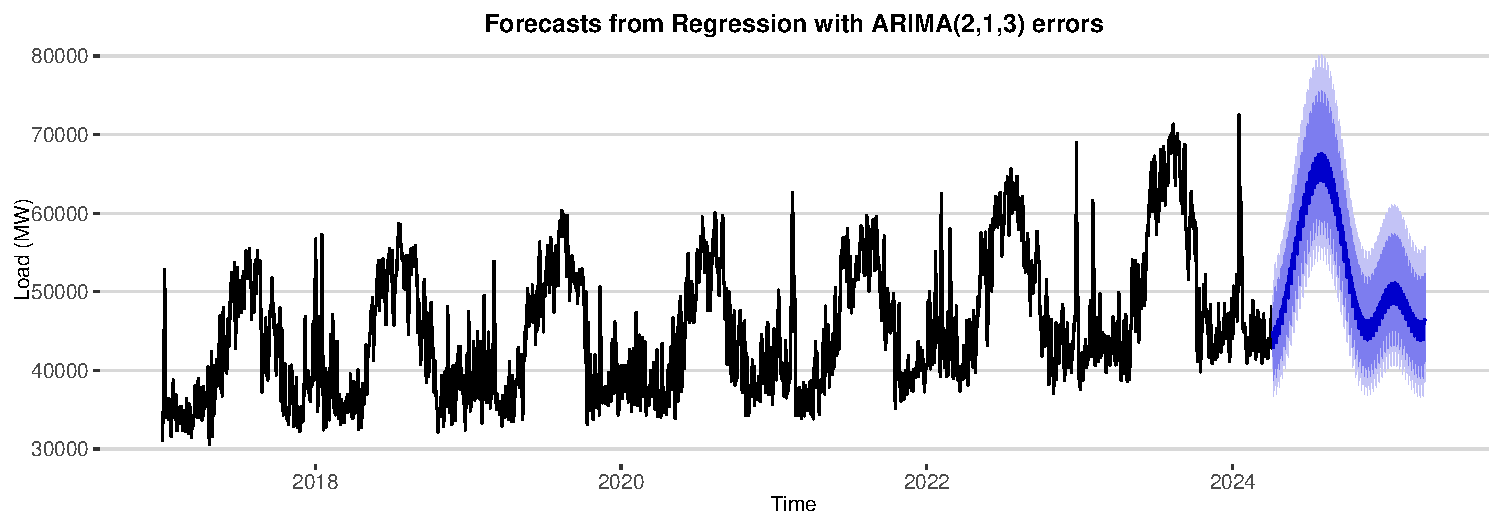
\includegraphics{FinalProject_Report_files/figure-latex/unnamed-chunk-8-1.pdf}
\caption{Forecasting Results from ARIMA+Fourier with K=c(2,3)}
\end{figure}

\begin{figure}
\centering
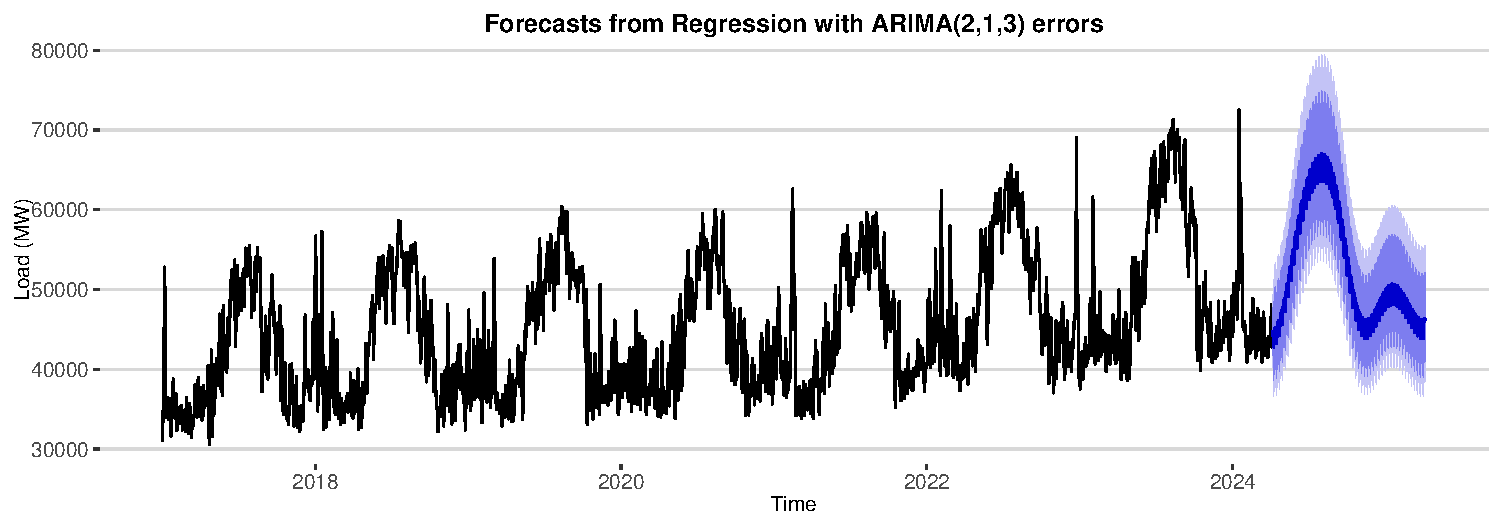
\includegraphics{FinalProject_Report_files/figure-latex/unnamed-chunk-9-1.pdf}
\caption{Forecasting Results from ARIMA+Fourier with K=c(2,4)}
\end{figure}

\begin{figure}
\centering
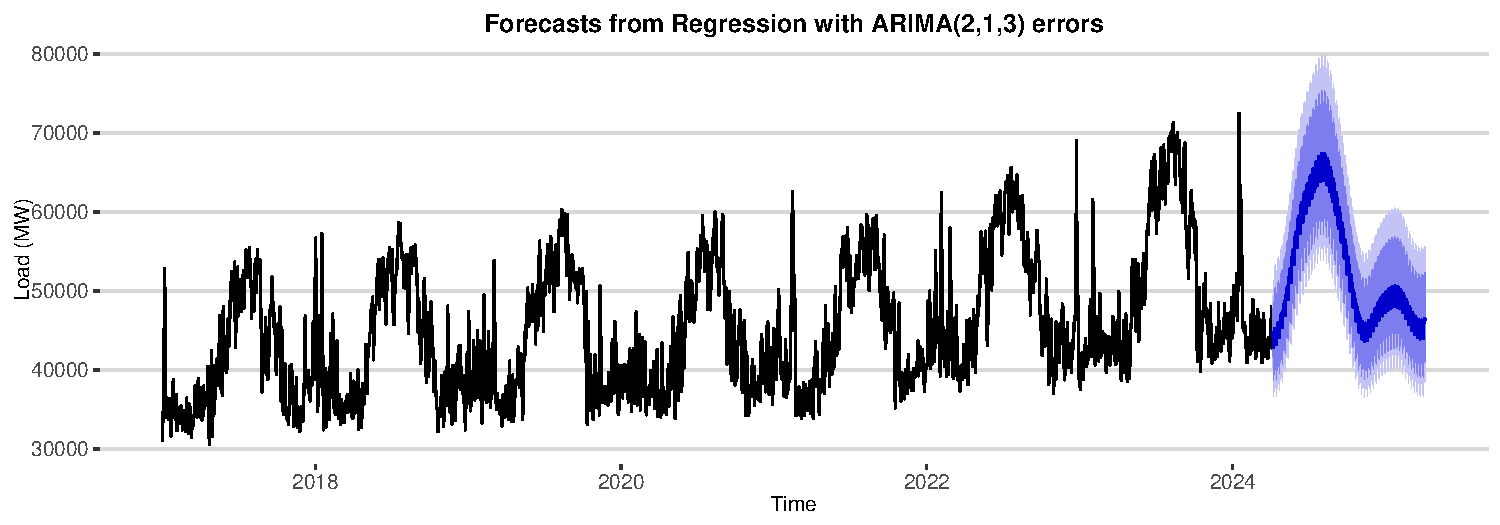
\includegraphics{FinalProject_Report_files/figure-latex/unnamed-chunk-10-1.pdf}
\caption{Forecasting Results from ARIMA+Fourier with K=c(2,6)}
\end{figure}

\begin{figure}
\centering
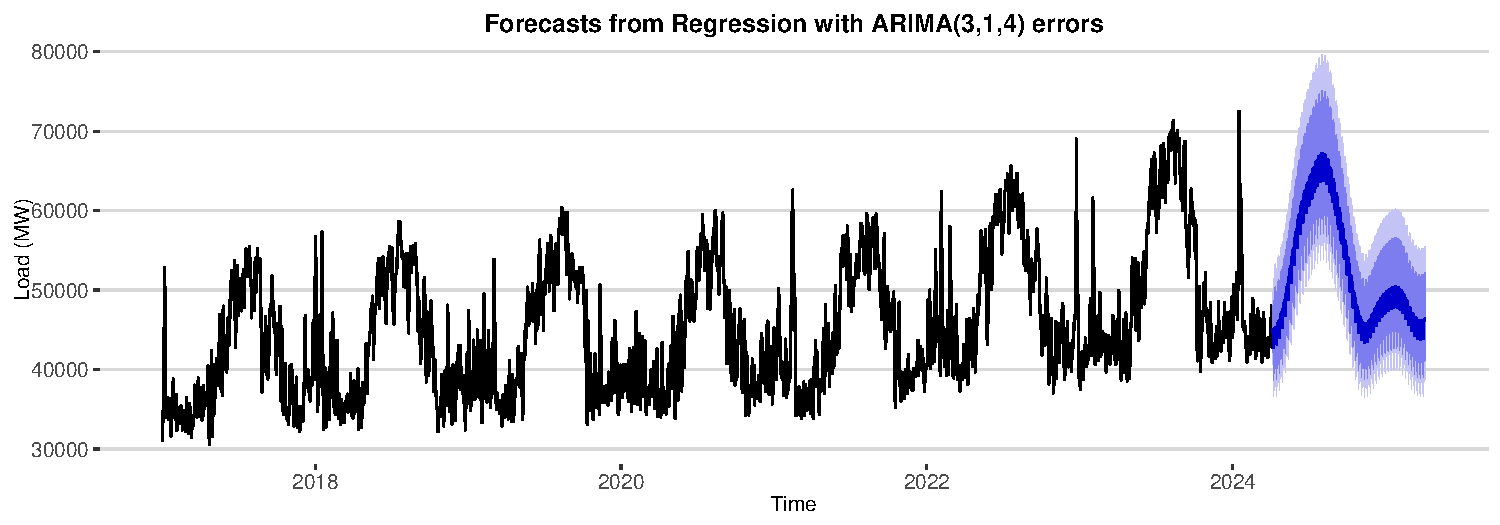
\includegraphics{FinalProject_Report_files/figure-latex/unnamed-chunk-11-1.pdf}
\caption{Forecasting Results from ARIMA+Fourier with K=c(3,6)}
\end{figure}

\begin{figure}
\centering
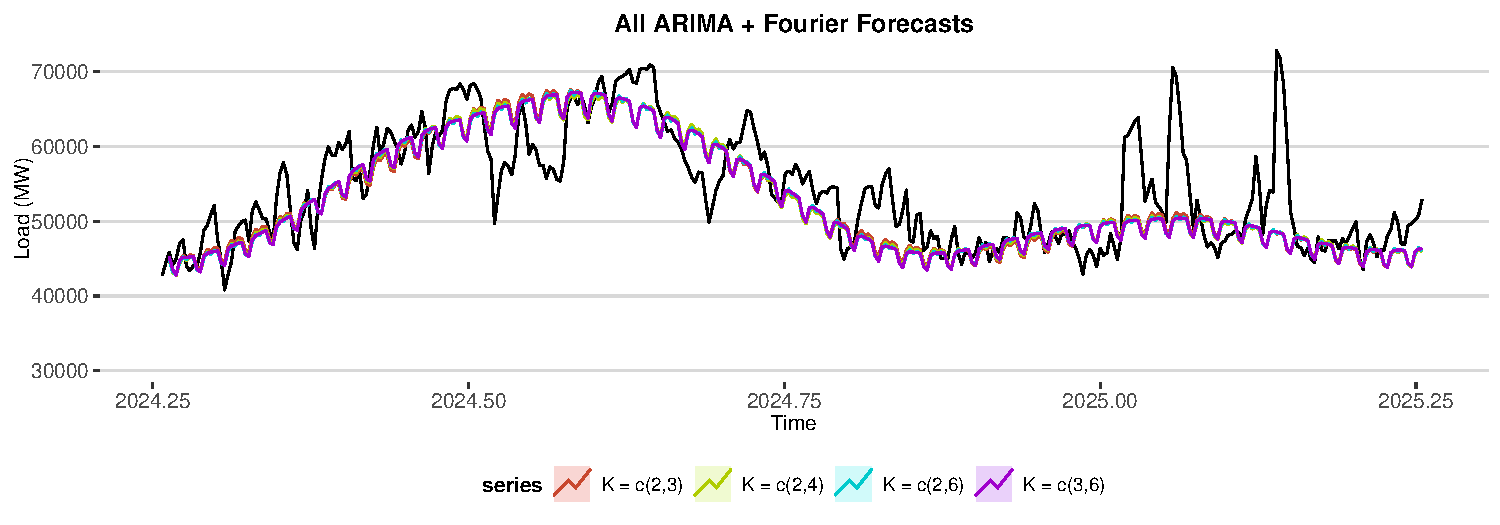
\includegraphics{FinalProject_Report_files/figure-latex/unnamed-chunk-12-1.pdf}
\caption{Observed Data and Forecasting Results from AF23, AF24, AF26,
AF36 Models}
\end{figure}

\newpage

\subsubsection{Neural Networks}\label{neural-networks}

Neural networks incorporate lagged values and Fourier terms as inputs to
model complex time series like ERCOT load data. They excel at capturing
non-linear relationships that traditional linear models (like ARIMA) may
struggle with. By using historical load patterns and multiple seasonal
indicators, neural networks can adapt to complex seasonal behaviors,
including interactions between short-term and long-term effects. The
inclusion of lagged inputs (p) and seasonal lags (P) allows the neural
network to model both short- and long-term dependencies, making it
analogous to SARIMA models, but with the added advantage of capturing
non-linearity.

For our three Neural Network models, we used the following K parameters:
K=c(2,4); K=c(2,6); and K=c(3,6). This means that there are 12, 16, and
18 total exogenous regressors modeled by Fourier terms, respectively. In
each neural network model, the autoregressive parameters were set to p=1
and P=1. Each model therefore incorporates the most recent observation
and one seasonal observation. This allows the models to learn both
short-term dependencies (like immediate trends or sudden spikes) and
long-term seasonal structure (like daily or weekly cycles). Combined
with the Fourier terms, this structure enhances the model's ability to
capture the complex, non-linear, and multi-seasonal behavior
characteristic of ERCOT load data.

\begin{figure}
\centering
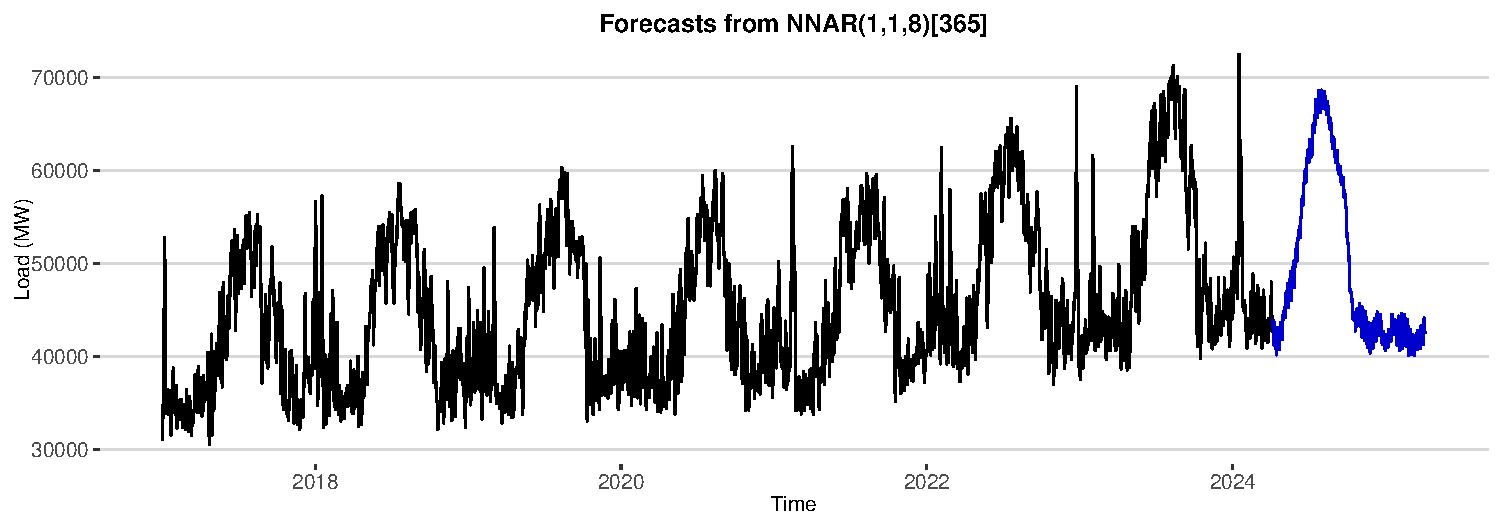
\includegraphics{FinalProject_Report_files/figure-latex/unnamed-chunk-13-1.pdf}
\caption{Forecasting Results from Neural Network with K=c(2,4)}
\end{figure}

\begin{figure}
\centering
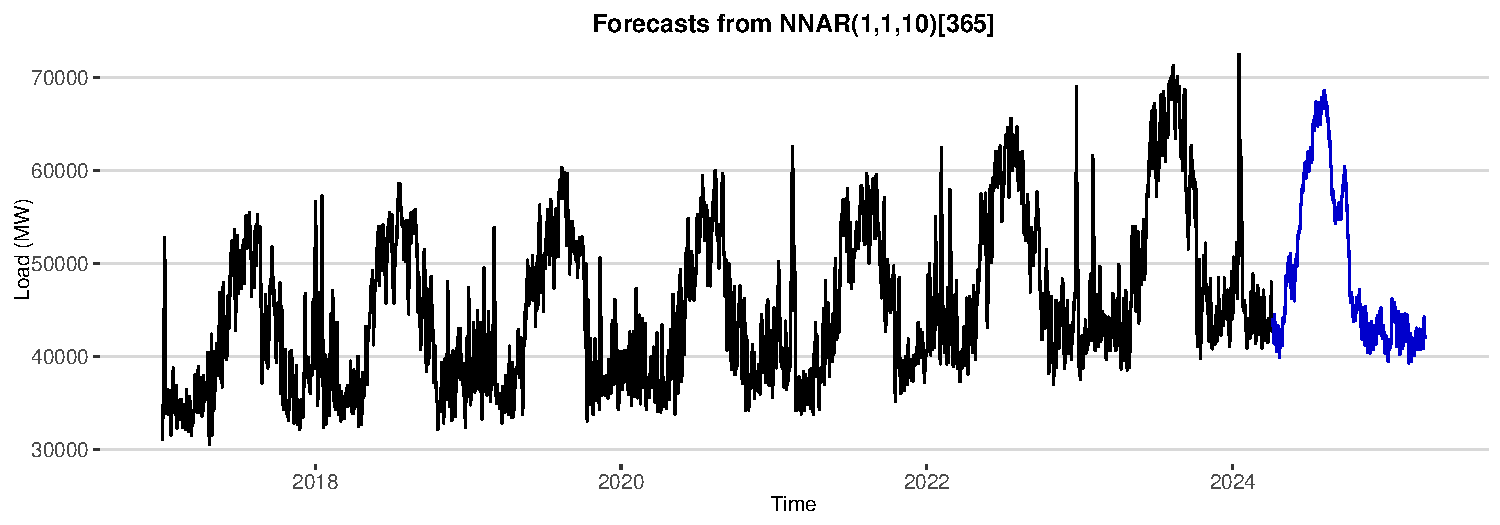
\includegraphics{FinalProject_Report_files/figure-latex/unnamed-chunk-14-1.pdf}
\caption{Forecasting Results from Neural Network with K=c(2,6)}
\end{figure}

\begin{figure}
\centering
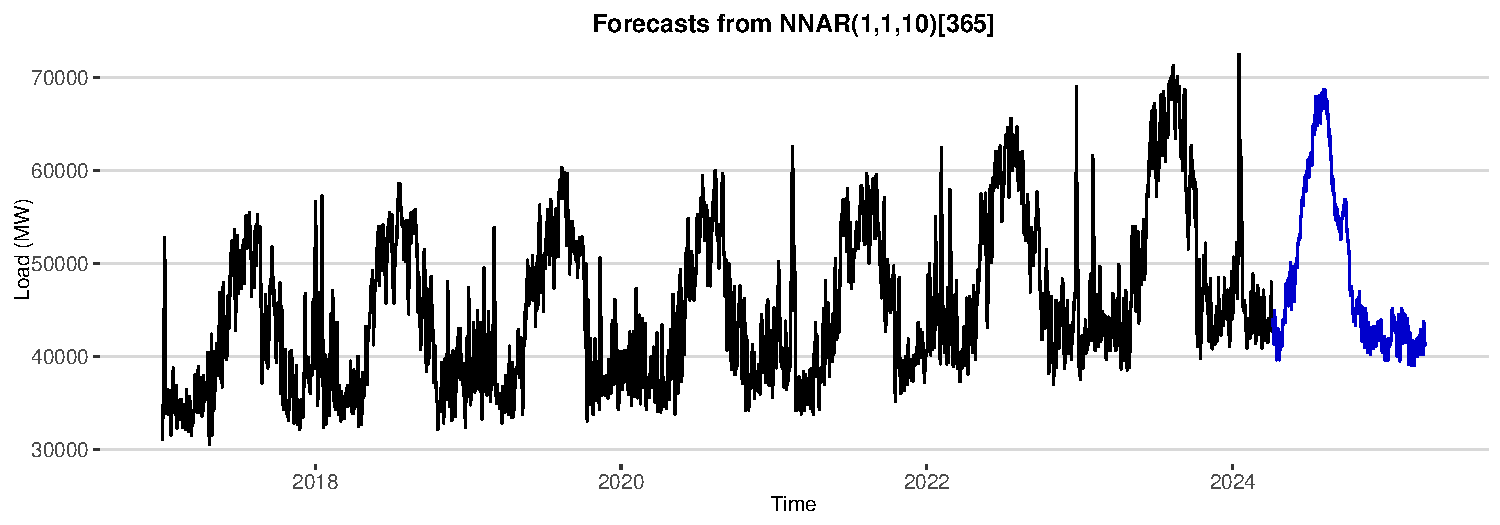
\includegraphics{FinalProject_Report_files/figure-latex/unnamed-chunk-15-1.pdf}
\caption{Forecasting Results from Neural Network with K=c(3,6)}
\end{figure}

\begin{figure}
\centering
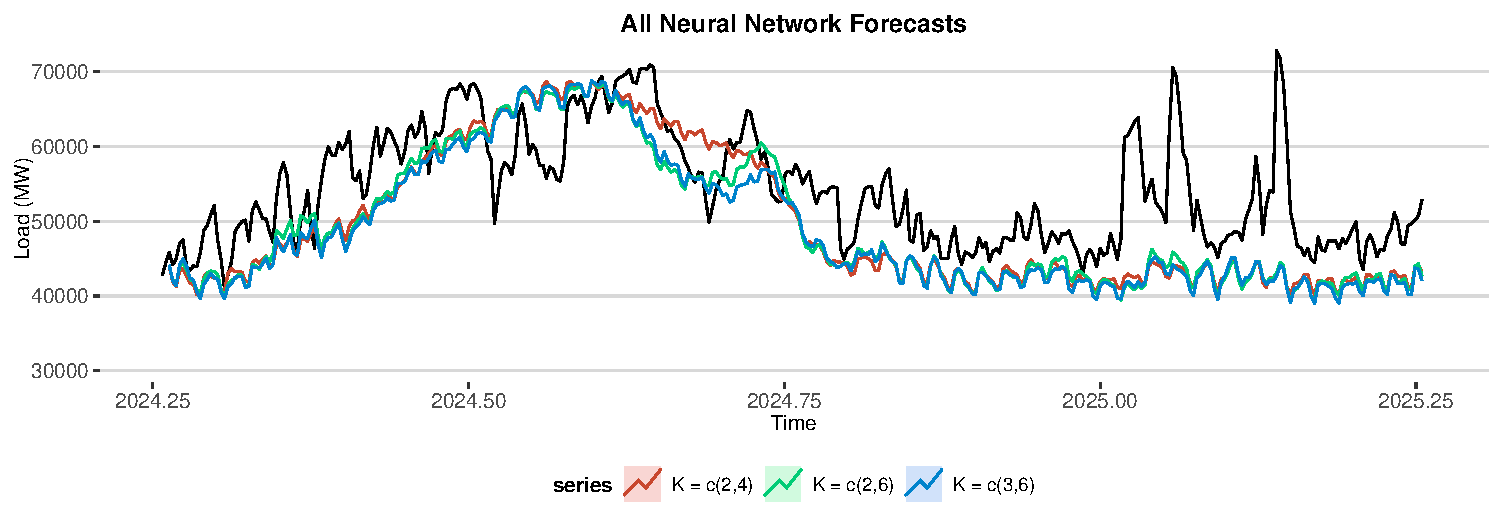
\includegraphics{FinalProject_Report_files/figure-latex/unnamed-chunk-16-1.pdf}
\caption{Observed Data and Forecasting Results from NN24, NN26, NN36
Models}
\end{figure}

\newpage

\subsection{Models with Monthly Data}\label{models-with-monthly-data}

\subsubsection{Seasonal ARIMA}\label{seasonal-arima}

The seasonal ARIMA (SARIMA) autofits single-seasonality patterns through
differencing and autoregressive/moving average components. This model is
suitable when ERCOT load displays dominant recurring seasonal trends.
Although it cannot model multiple seasonalities simultaneously, SARIMA
remains a strong baseline for data with clear, stable seasonal
structure.

\begin{figure}
\centering
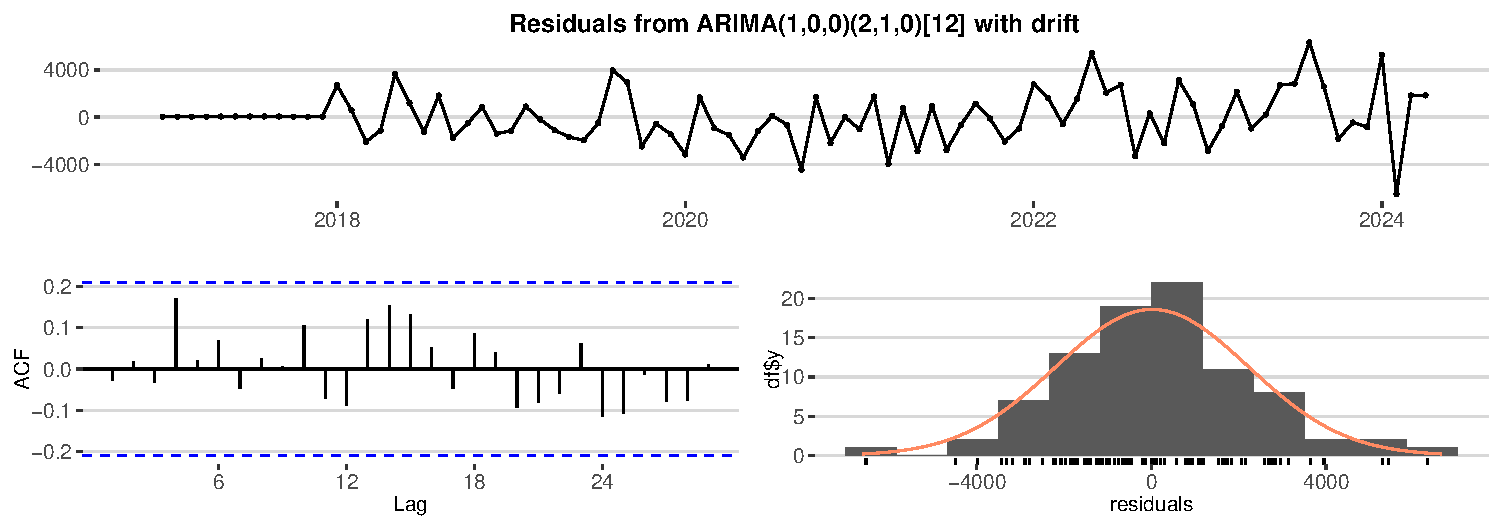
\includegraphics{FinalProject_Report_files/figure-latex/unnamed-chunk-17-1.pdf}
\caption{Residuals (SARIMA)}
\end{figure}

\begin{verbatim}
## 
##  Ljung-Box test
## 
## data:  Residuals from ARIMA(1,0,0)(2,1,0)[12] with drift
## Q* = 13.485, df = 15, p-value = 0.5649
## 
## Model df: 3.   Total lags used: 18
\end{verbatim}

\begin{figure}
\centering
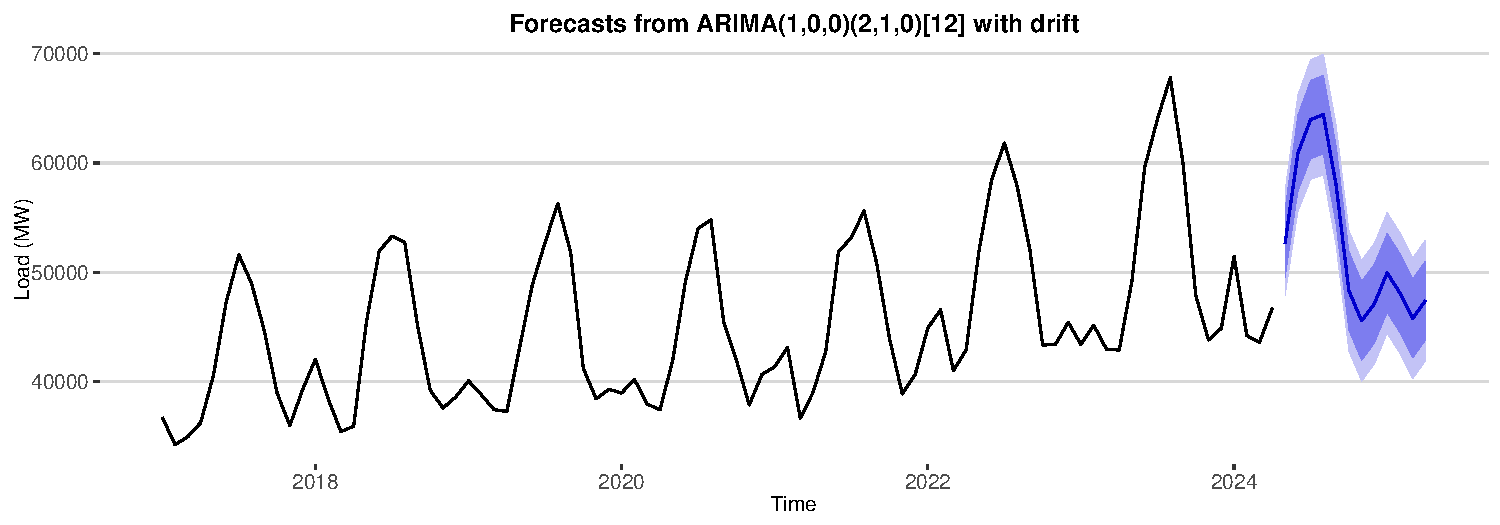
\includegraphics{FinalProject_Report_files/figure-latex/unnamed-chunk-18-1.pdf}
\caption{Forecasting Results from SARIMA}
\end{figure}

\newpage

\subsubsection{State Space Exponential
Smoothing}\label{state-space-exponential-smoothing}

State Space Exponential Smoothing (SSES) offers a probabilistic and
flexible approach to forecasting, modeling uncertainty while capturing
both trend and seasonality. It automatically selects among additive or
multiplicative trend and seasonal components based on the data, making
it well-suited for monthly ERCOT load data where seasonal strength and
trend can evolve over time. Its ability to model uncertainty and
structural changes without manual re-specification is especially useful
when trying to capture varying patterns.

\begin{figure}
\centering
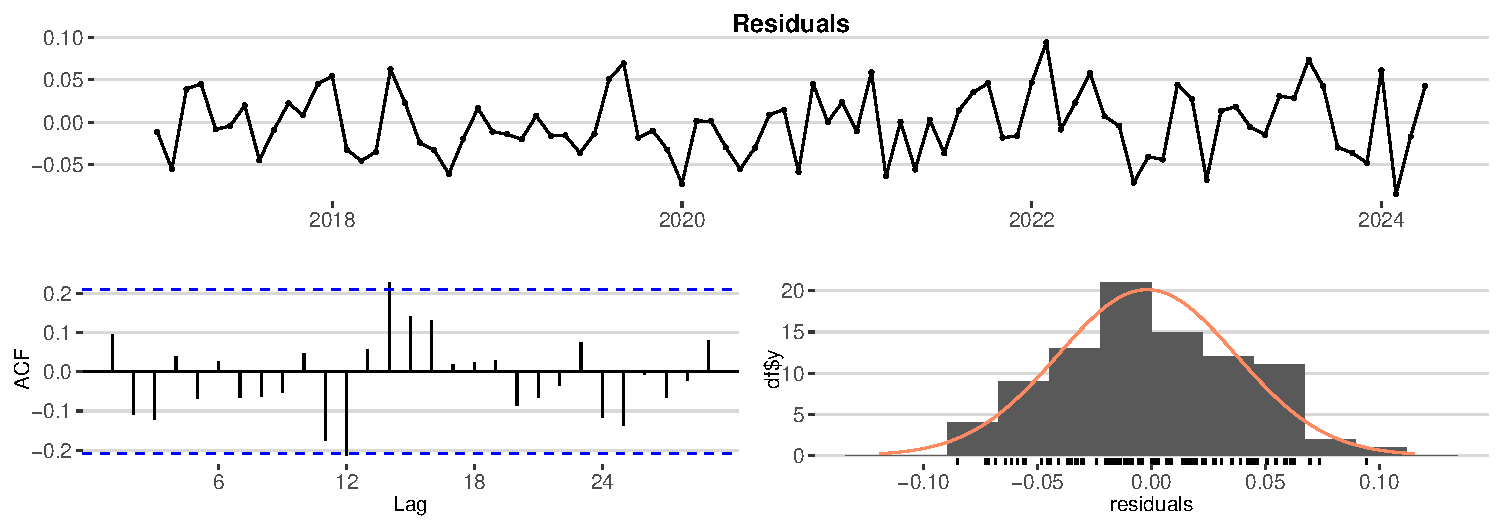
\includegraphics{FinalProject_Report_files/figure-latex/unnamed-chunk-19-1.pdf}
\caption{Residuals (SSES)}
\end{figure}

\begin{verbatim}
## 
##  Ljung-Box test
## 
## data:  Residuals
## Q* = 23.142, df = 18, p-value = 0.1852
## 
## Model df: 0.   Total lags used: 18
\end{verbatim}

\begin{figure}
\centering
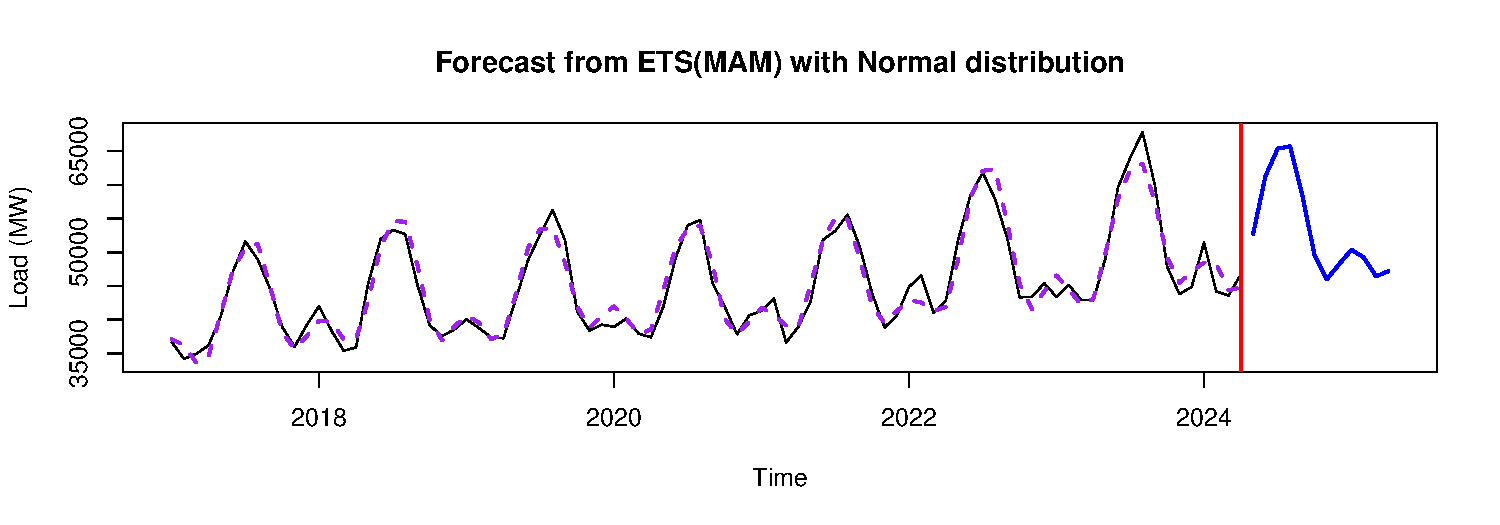
\includegraphics{FinalProject_Report_files/figure-latex/unnamed-chunk-20-1.pdf}
\caption{Forecasting Results from SS Exponential Smoothing}
\end{figure}

\newpage

\subsubsection{Structural Bayesian State Space
Model}\label{structural-bayesian-state-space-model}

Structural Bayesian State Space Model (SSBSM) is also a probabilistic
framework, and it assumes that all components (trend, seasonality,
irregularity) are stochastic and can evolve over time. This allows each
element to change dynamically, providing robustness in the face of
structural shifts due to climate variability, policy changes, or
demand-side management. For monthly ERCOT load forecasting, this model
is a suitable option when long-term patterns are not fixed and may
change unpredictably.

\begin{figure}
\centering
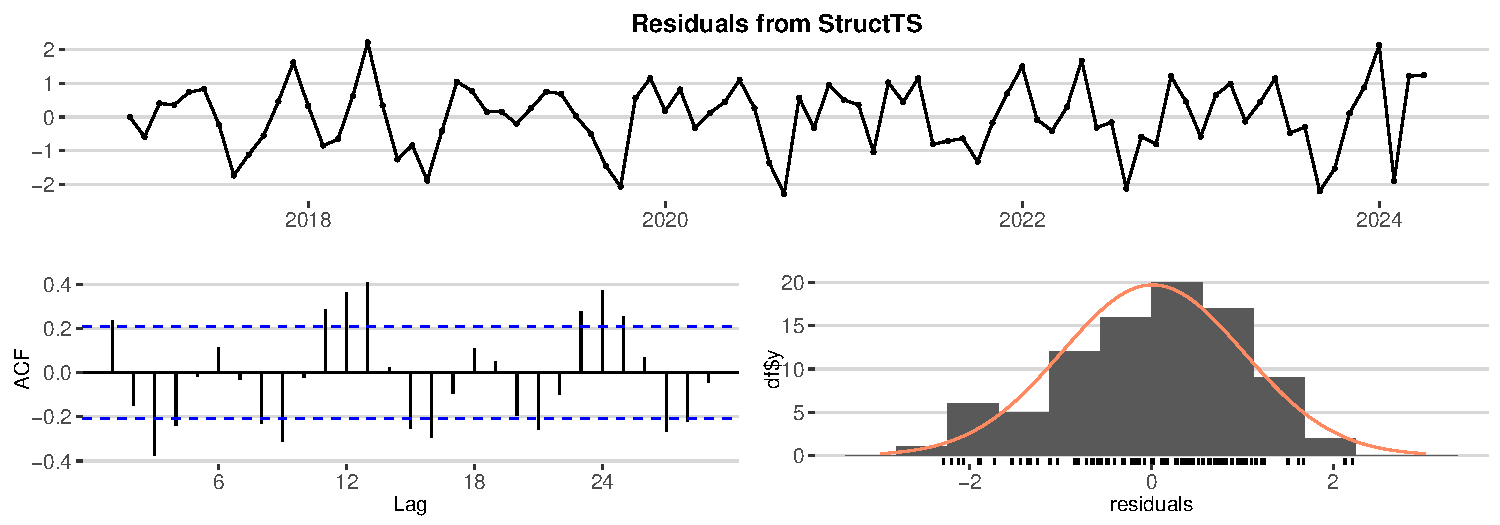
\includegraphics{FinalProject_Report_files/figure-latex/unnamed-chunk-21-1.pdf}
\caption{Residuals (SSBSM)}
\end{figure}

\begin{verbatim}
## 
##  Ljung-Box test
## 
## data:  Residuals from StructTS
## Q* = 100.29, df = 18, p-value = 1.961e-13
## 
## Model df: 0.   Total lags used: 18
\end{verbatim}

\begin{figure}
\centering
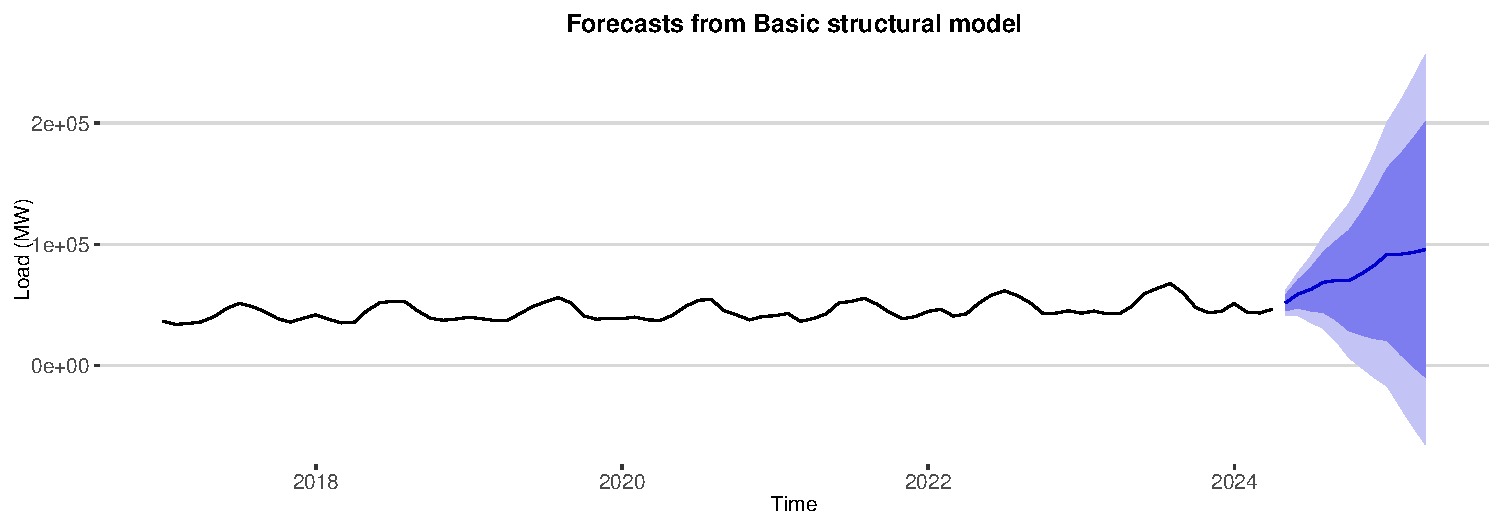
\includegraphics{FinalProject_Report_files/figure-latex/unnamed-chunk-22-1.pdf}
\caption{Forecasting Results from SS Basic Structure Model}
\end{figure}

\subsubsection{Scenario Generation}\label{scenario-generation}

Lastly, we did scenario generation using Cholesky decomposition, which
allowed us to create multiple realistic future ERCOT load forecasts by
simulating correlated input variables. First, we calculate the
historical covariance matrix of the load and the 7 predictors. Then,
using Cholesky decomposition, we broke this matrix into a lower
triangular matrix that captures the variables' dependencies. By
multiplying random normal samples by this matrix, we generated new input
scenarios that preserve historical correlations. These are then fed into
an ARIMA + Fourier forecasting model to produce a range of potential
load trajectories. Doing this helps to capture uncertainty in both the
predictors and their influence on load.

\begin{figure}
\centering
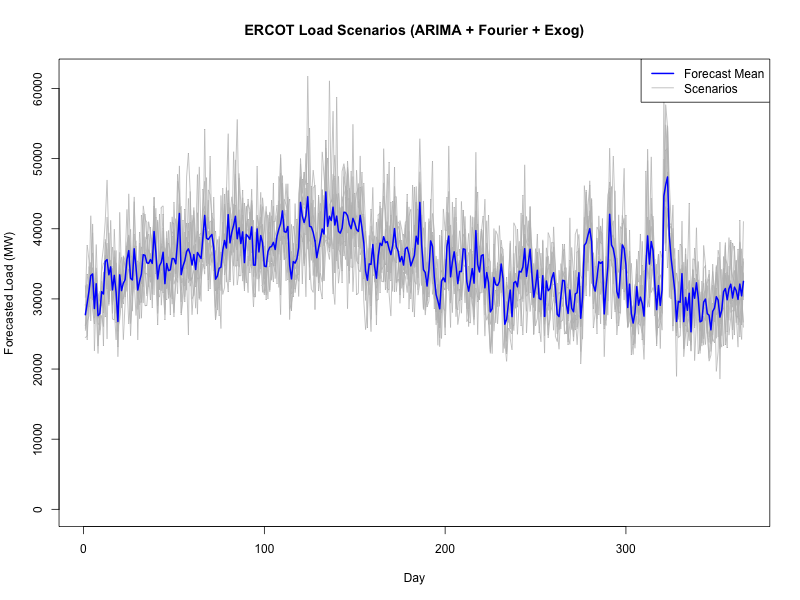
\includegraphics{ercot_load_scenarios.png}
\caption{ERCOT Load Scenario Generation}
\end{figure}

This ARIMA + Fourier + exogenous variables model with Cholesky-based
scenario generation shows overall trends well, but it doesn't seem to
capture large spikes in load that we were expecting (i.e.~more values in
the 60-70 GW range). The scenarios mostly stay close to the mean of the
original data set and don't reflect the more extreme values we sometimes
see in actual data. This might be because Cholesky decomposition uses a
multivariate normal distribution, which keeps the correlations between
variables but tends to produce values clustered around the average,
without many extreme highs or lows.

\newpage

\section{Results and Model
Comparisons}\label{results-and-model-comparisons}

\begin{table}[!h]
\centering
\caption{\label{tab:unnamed-chunk-24}Forecast Accuracy for Load}
\centering
\begin{tabular}[t]{l|r|r|r|r|r|r|r}
\hline
Model & ME & RMSE & MAE & MPE & MAPE & ACF1 & Theil's U\\
\hline
NN24 & 4362.752 & 7731.014 & 6161.221 & 8.08616 & 11.27736 & 0.91331 & 2.66029\\
\hline
NN26 & 5245.005 & 7752.327 & 6367.270 & 9.54623 & 11.51576 & 0.88995 & 2.64404\\
\hline
NN36 & 4393.755 & 7606.073 & 6084.019 & 8.14946 & 11.16011 & 0.90554 & 2.62815\\
\hline
SARIMA & 1891.987 & 3125.671 & 2638.377 & 3.61048 & 4.86036 & -0.06288 & 0.59759\\
\hline
SSES & 1183.083 & 2929.559 & 2383.270 & 2.31508 & 4.38636 & -0.02696 & 0.55750\\
\hline
SSBM & -21702.918 & 28172.579 & 22554.935 & -42.77079 & 44.23444 & 0.81247 & 5.64407\\
\hline
STL+ETS & 4320.595 & 6453.940 & 4992.943 & 7.57688 & 8.85220 & 0.83777 & 2.13999\\
\hline
TBATS & 2905.599 & 5794.056 & 4369.840 & 5.03801 & 7.80851 & 0.86071 & 1.94380\\
\hline
AF23 & 1458.268 & 5148.588 & 3746.586 & 2.31101 & 6.68713 & 0.85424 & 1.72536\\
\hline
AF24 & 1521.098 & 5166.958 & 3756.300 & 2.42856 & 6.70843 & 0.85414 & 1.73282\\
\hline
AF26 & 1545.030 & 5166.779 & 3745.856 & 2.47411 & 6.68810 & 0.85374 & 1.73143\\
\hline
AF36 & 1514.696 & 5155.774 & 3732.166 & 2.41897 & 6.66264 & 0.85621 & 1.72704\\
\hline
\end{tabular}
\end{table}

According to the forecast accuracy metrics of our models, particularly
the Mean Absolute Percentage Error (MAPE), the best model for
forecasting daily load was the ARIMA + Fourier terms model with K
parameter K=c(3,6), the Fourier terms representing 18 exogenous
regressors. The best model for forecasting monthly load was the State
Space Exponential Smoothing model, closely followed by the SARIMA model.

\begin{figure}
\centering
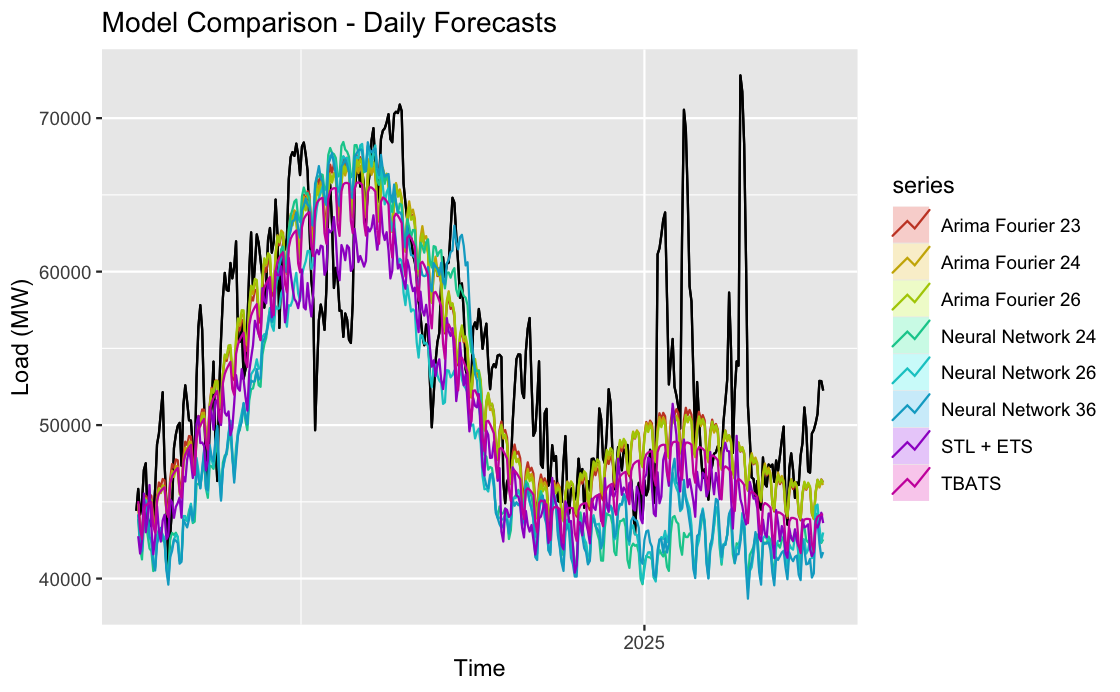
\includegraphics{model_comparison_daily.png}
\caption{Comparison of Models Used to Forecast Daily Load}
\end{figure}

After plotting the forecasting models for daily load, with actual test
load data shown in black, it appears that the models failed to capture
large swings in daily load. Despite this, visually, it looks like the
models performed well in capturing the general trends and seasonality of
the daily load data.

\begin{figure}
\centering
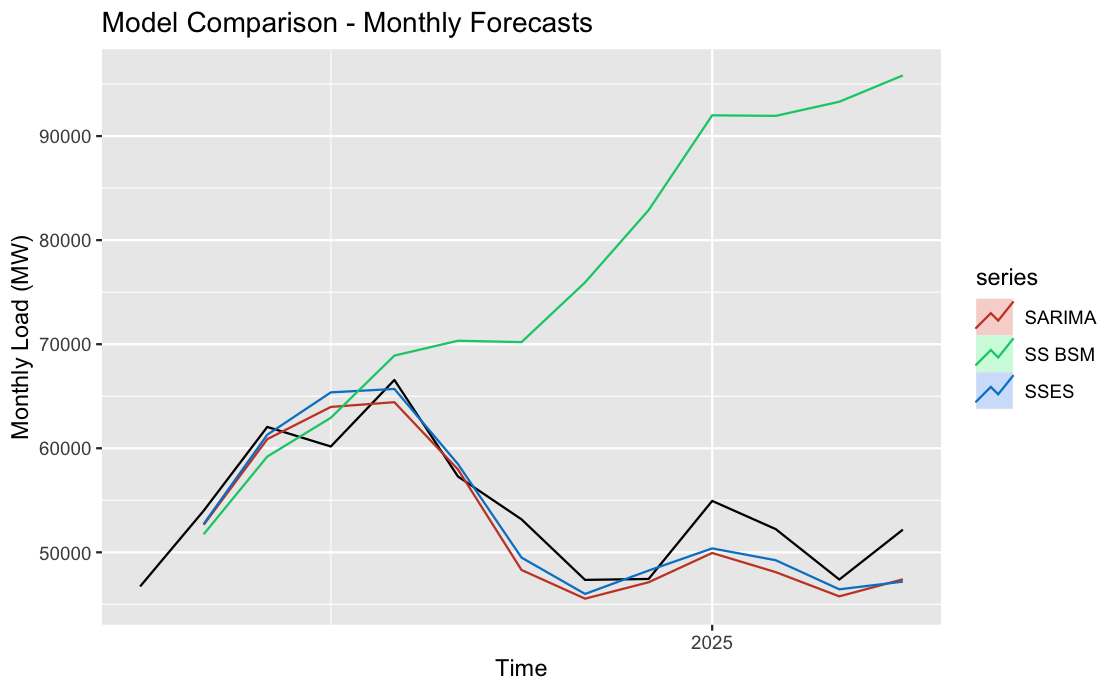
\includegraphics{model_comparison_monthly.png}
\caption{Comparison of Models Used to Forecast Monthly Load}
\end{figure}

Compared to the forecasting models for daily load, from only looking at
the plot, the forecasting models for monthly load appear to have
performed better (with the exception of the SSBSM model). The SARIMA and
SSES models exhibit a very similar trend and seasonality to that of the
test load data in black. In contrast, the SSBSM model appears to diverge
strongly from what is expected to occur, which suggests it may be
extrapolating a certain trend too aggressively.

\newpage

\section{Conclusions}\label{conclusions}

According to the results of our models, we can conclude that daily
forecasting improves with more flexible approaches like ARIMA with
Fourier terms and non-linear models like Neural Networks, which can
adapt to short-term variability and capture complex patterns in the
data. Simpler and more stable models like SARIMA and SSES are more
effective for monthly forecasting, as they generalize better over longer
horizons with less overfitting.

For scenario generation, Cholesky decomposition offers a straightforward
way to create realistic-looking variations by preserving the correlation
structure in the data. However, it tends to produce values clustered
around the mean and struggles to represent rare, high-impact events like
extreme load spikes. This could limit its usefulness in stress-testing
or planning for outlier conditions, which are increasingly important in
energy systems under more volatile conditions.

Load forecasting is an important tool for power system planning and
operation. Accurate forecasts help grid operators have a reliable
balance between electricity supply and demand, avoid blackouts, and
minimize operational costs. They also support market participants in
making decisions about bidding and generation schedules. As the grid
becomes more complex and dynamic with increasing renewable integration,
extreme weather events, and changing consumption patterns, flexible
forecasting methods become even more essential for maintaining grid
reliability and efficiency.

\section{References}\label{references}

\begin{enumerate}
\def\labelenumi{\arabic{enumi}.}
\item
  Guo, Kayla. Data centers are booming in Texas. What does that mean for
  the grid? Published 24 Jan.~2025.
  \url{https://www.texastribune.org/2025/01/24/texas-data-center-boom-grid/}.
\item
  Kleckner, Tom. Batteries, Solar Help ERCOT Meet Record Winter Peak, 20
  Feb.~2025,
  \url{https://www.rtoinsider.com/98816-batteries-solar-help-ercot-meet-record-winter-peak/}.
\item
  Walton, Robert. ``US Electricity Load Growth Forecast Jumps 81\% Led
  by Data Centers, Industry: Grid Strategies.'' Utility Dive, 13
  Dec.~2023,
  www.utilitydive.com/news/electricity-load-growing-twice-as-fast-as-expected-Grid-Strategies-report/702366/.
\item
  Zimmerman, Zach, and John D Wilson. The Era of Flat Power Demand Is
  Over, Dec.~2023,
  gridstrategiesllc.com/wp-content/uploads/2023/12/National-Load-Growth-Report-2023.pdf.
\end{enumerate}

\section{Acknowledgment of AI
Assistance}\label{acknowledgment-of-ai-assistance}

\emph{ChatGPT was used for troubleshooting code syntax and working
through sections of scenario generation as this was newer material. All
models and forecasts were executed and validated locally in RStudio by
the authors.}

\end{document}
